%\documentclass[conference]{IEEEtran}
%\IEEEoverridecommandlockouts
%\usepackage[english]{babel}

\documentclass[12pt]{article}
\usepackage[letterpaper,top=2cm,bottom=3cm,left=2cm,right=2cm,marginparwidth=1.75cm]{geometry}


% Set page size and margins
% Replace `letterpaper' with `a4paper' for UK/EU standard size

\usepackage{doi}
\bibliographystyle{apalike}

\usepackage{subcaption} 
\usepackage{enumitem}
\usepackage{threeparttable}

\usepackage{graphicx}
\graphicspath{{figures/}}   % filled by paper/collect_figures.sh from outputs/
\usepackage{amssymb}
\usepackage{amsmath}
\usepackage{dsfont}
\usepackage{xurl}

\usepackage{tikz}
\usetikzlibrary{arrows,automata,backgrounds,fit,patterns,petri,shadows,shapes}
\pgfdeclarepatternformonly{stripes}
{\pgfpointorigin}{\pgfpoint{0.25cm}{0.25cm}}
{\pgfpoint{0.25cm}{0.25cm}}
{
    \pgfpathmoveto{\pgfpoint{0cm}{0cm}}
    \pgfpathlineto{\pgfpoint{0.25cm}{0.25cm}}
    \pgfpathlineto{\pgfpoint{0.25cm}{0.12cm}}
    \pgfpathlineto{\pgfpoint{0.12cm}{0cm}}
    \pgfpathclose%
    \pgfusepath{fill}
    \pgfpathmoveto{\pgfpoint{0cm}{0.12cm}}
    \pgfpathlineto{\pgfpoint{0cm}{0.25cm}}
    \pgfpathlineto{\pgfpoint{0.12cm}{0.25cm}}
    \pgfpathclose%
    \pgfusepath{fill}
}

\usepackage{comment}
\usepackage{array}
\usepackage{booktabs}
\usepackage{bm}

\usepackage{hyperref}
\hypersetup{breaklinks=true,
    pdftitle={Optimal incentive schemes to enhance colorectal cancer screening participation}} 


\tikzstyle{decisionPM} = [rectangle, draw, thick, minimum size = 0.8cm, fill = green!20]
\tikzstyle{decisionC} = [rectangle, draw, thick, minimum size=0.8cm, fill = yellow!20]
\tikzstyle{decisionSP} = [rectangle, draw, thick, minimum size=0.8cm, fill = blue!20]
\tikzstyle{decisionF} = [rectangle, draw, thick, minimum size=0.8cm, fill = orange!20]
\tikzstyle{determ} = [circle, draw, thick, double, minimum size = 0.8cm]
\tikzstyle{chance} = [circle, thick, minimum size = 0.8cm, inner sep= 1pt, draw = black, pattern = stripes, pattern color = gray!40]
\tikzstyle{chanceD} = [circle, thick, minimum size = 0.8cm, inner sep= 1pt, draw = black, fill=green!20]
\tikzstyle{chanceA} = [circle, thick, minimum size = 0.8cm, inner sep= 1pt, draw = black, fill = yellow!20]


\tikzstyle{utilityPM} = [regular polygon, regular polygon sides = 6, draw, inner sep= 1pt, thick, minimum size=0.8cm, fill = green!20]
\tikzstyle{utilityC} = [regular polygon, regular polygon sides = 6, draw, inner sep= 1pt, thick, minimum size=0.8cm, fill = yellow!20]
\tikzstyle{utilitySP} = [regular polygon, regular polygon sides = 6, draw, inner sep= 1pt, thick, minimum size=0.8cm, fill = blue!20]
\tikzstyle{utilityF} = [regular polygon, regular polygon sides = 6, draw, inner sep= 1pt, thick, minimum size=0.8cm, fill = orange!20]
\tikzstyle{arrow} = [thick,->,>=stealth]


%\usepackage{cite}
\usepackage{amsmath,amssymb,amsfonts}
\usepackage{algorithmic}
\usepackage{graphicx}
\usepackage{textcomp}
\usepackage{xcolor}
\def\BibTeX{{\rm B\kern-.05em{\sc i\kern-.025em b}\kern-.08em
    T\kern-.1667em\lower.7ex\hbox{E}\kern-.125emX}}
\usepackage[round]{natbib}
\usepackage{enumitem}

% ---- review marks (revision of 2026-11): \reviewfalse gives the clean version ----
\newif\ifreview \reviewtrue
\newcommand{\rev}[1]{\ifreview{\color{blue}#1}\else#1\fi}
\newcommand{\revdel}[1]{\ifreview{\color{red}\footnotesize[deleted: #1]}\fi}
\newcommand{\revtodo}[1]{\ifreview{\color{orange}\textbf{[TODO: #1]}}\fi}

\begin{document}

\title{Optimal incentive schemes to enhance colorectal cancer screening participation\thanks{Work supported by the AXA-ICMAT Chair in Adversarial Risk Analysis; the Spanish Ministry of Science project PID2025-1724120B-C21; Grant CEX2023-001347-S funded by MICIU/AEI/10.13039/501100011033; the European Union's Horizon 2020 Research and Innovation Programme under Grant Agreement N. 101097036 (ONCOSCREEN); and the European Commission – NextGenerationEU, through the Momentum CSIC Programme: Develop Your Digital Talent}
}

%\author{\IEEEauthorblockN{Daniel Corrales}
%\IEEEauthorblockA{\textit{Mathematical Sciences Institute, ICMAT-CSIC}\\
%Madrid, Spain daniel.corrales@icmat.es}
%\and
%\IEEEauthorblockN{David Rios Insua}
%\IEEEauthorblockA{\textit{Mathematical Sciences Institute, ICMAT-CSIC}\\
%Madrid, Spain david.rios@icmat.es}
%}

%\author{Daniel Corrales \\
%ICMAT-CSIC \and David Rios Insua \\ ICMAT-CSIC}
\author{}
\date{ONGOING WORK WITHIN ONCOSCREEN PROJECT.\\ DO NOT CIRCULATE}

\maketitle
\begin{abstract}
Colorectal cancer is a major cause of death worldwide despite being a disease with a high survival rate if detected early. Numerous screening protocols, mainly based on age, have been designed to avoid the consequences of cancer development in citizens. However, participation in these programmes tends to remain far below the desired levels. This work studies how a policymaker should design policies to raise screening participation when it does not know the preferences and beliefs of the citizens it seeks to influence. Using adversarial risk analysis, the policymaker forecasts participation from citizens who differ in how they weigh the future, perceive their risk and bear the burden of screening, and then chooses a maximum expected utility policy. The approach is applied to a public scheme, in which the policymaker pays the citizen directly, and a private-public scheme, in which a provider runs the programme and the policymaker must also forecast the provider's campaign. Applied to faecal immunochemical test screening on Spanish records, inviting citizens by assessed risk rather than age is a robust gain, and a common financial incentive to citizens \rev{adds less, and}\revdel{also has a large effect but} depends on how strongly participation responds to money and citizens' attitude towards risk. The public-private contract improves on the public scheme mainly through support for citizen's access to the test\rev{, even when the policymaker is uncertain about the effect of that support and about the provider's costs and attitude to risk}.
\end{abstract}

\begin{small}
\textbf{Keywords}: Colorectal cancer, screening, incentives, decision analysis, public-private partnerships.     
\end{small}



%%%%%%%%%%%%%%%%%%%%%%%%%%%%%%%%%%%%%%%%%%%%%%%%%
\section{Introduction}\label{intro}
 
Colorectal cancer (CRC) is the third most common type of cancer worldwide, making up about 10\% of all cancer cases \citep{WHO} and accounting for approximately 12\% of all cancer-associated deaths. In 2020, there were 1.9 million new cases and 930,000 associated deaths worldwide \citep{morgan2023global}. \rev{In the EU alone}\revdel{Just in the EU}, its estimated annual costs in 2015 were approximately 19 B€ \citep{henderson2021economic}. Importantly, the societal costs associated with late-stage detection have proved higher than those related to early-stage detection \citep{mar2017cost}.

Despite this, only a relatively small percentage of invited susceptible EU citizens participate in screening programmes, which currently mostly use one-size-fits-all strategies based on age and rely on faecal testing, which is cheap and comfortable but \rev{of limited accuracy}\revdel{not very accurate}. If test results are positive, colonoscopy is recommended, which is highly accurate but expensive, uncomfortable, and carries a risk of serious complications. Even when screening is in their best interests, many citizens do not attend, for reasons including lack of information, inappropriate communication, aversion to the screening methods, or risk misestimation \citep{KASTRINOS}. Hence, there is a need for: i) accurate, non-invasive, cost-effective screening tests based on novel technologies; ii) raising further awareness about the disease and the relevance of its early detection; iii) introducing personalised screening approaches covering genetic and socioeconomic factors as well as environmental stressors that potentially lead to different disease onsets; and iv) designing policies to increase participation in screening programmes, such as incentive schemes, the subject of this paper.

The meta-analysis in \cite{facciorusso2021addition} concerning the impact of incentives to promote adherence to CRC screening programmes in the USA suggested a slightly positive impact, even though the incentives used were low. \cite{neuvonen2025optimizing} introduce a portfolio optimisation scheme to design screening programmes, including a yes/no decision concerning the introduction of a small (10€) scheme to promote participation. The approach we adopt here is different, as we aim at designing optimal incentives for a given screening procedure, comparing various incentive mechanisms and setting them against the choice of whom to invite. The basic idea is that incentives can induce better adherence to a screening programme and, consequently, lead to earlier detection of CRC cases, thus increasing disease survival rates and improving quality of life among CRC patients, which can compensate for the incentive costs.

Many public policies use such incentives, and their implementation shows that they must be designed with care. Too large incentives can strain public budgets. This is the case of Spain's early subsidies to solar energy, which had to be abruptly cut back when their cost became unsustainable \citep{del2012support}. Too small incentives hardly stimulate behaviour change. This may be the case of the 5€ incentives for CRC screening suggested in \cite{facciorusso2021addition}.

The problem we therefore face is determining optimal financial incentives from the point of view of a policymaker (PM) taking into account the behaviour of citizens (C).  In some of the schemes to be analysed, there will be a private third party, a designated service provider (SP), managing and implementing screening and incentive campaigns. In broad terms, the problem of designing policies can be understood as a game and, more specifically, as a principal-agent problem \citep{smith1997principal} where the PM is the principal and the citizens are viewed as agents. For reasons outlined in \cite{rios2009adversarial} and \cite{ARAoverview}, rather than adopting standard game-theoretic approaches typical of this domain, relying on Nash equilibria and related refinements, we pursue a decision analytic approach based on adversarial risk analysis (ARA). This is a methodology to support a decision maker under uncertainty in the presence of agents with different goals, which does not require their preferences and beliefs to be common knowledge \citep{raiffa2007negotiation}. In such a situation, the PM models the behaviour of the citizens to forecast their adherence and, accordingly, finds incentives that modify it. To showcase the flexibility of the methodology, we illustrate it with a purely {\em public scheme} involving two agents, and a public-private scheme involving three agents based on {\em outcome-based payments}.

Our contributions are threefold. First, we formulate the incentive design problem for CRC screening as an ARA problem, in which the PM forecasts participation from a random model of the citizens' preferences and beliefs, rather than assuming common knowledge. Second, we extend it to an outcome-based contract with a service provider, a three-agent problem in which the PM forecasts the provider's campaign and the provider forecasts the citizens' responses. Third, we apply both to Spanish FIT screening, comparing age- and risk-based invitation, a common incentive, and a contract under which the provider can vary incentives across groups and navigate or support the access of citizens who do not respond\rev{, and we assess how robust the contract is to the provider's attitude to risk, which the policymaker does not know}.

For this analysis, we draw on the database presented in Appendix \ref{app:models} as well as on earlier models for CRC prediction \citep{corrales2024colorectal} and screening \citep{corrales2025decision} summarised in the same appendix. Code to reproduce the models is available at \url{https://github.com/DanielCorralesAlonso/optimized_crc_incentives_ara}.

%%%%%%%%%%%%%%%%%%%%%%%%%%%%%%%%%%%%%%%%%%%%%%%%%%%%%%
\section{Incentives to increase screening participation} \label{sec:incentive_problem_definition}
Section \ref{sec:basic_setup} introduces the general problem setup, while Sections \ref{sec:public_scheme} and \ref{sec:OBP} define the theoretical framework for the public scheme and the public-private scheme, respectively. Throughout, subscripts name the agent holding a belief or a preference; $\pi$ denotes an agent's forecast of another agent's decision; $U$, $P$ and $\Psi$ denote the random counterparts of $u$, $p$ and $\psi$ with which one agent models another; and bold symbols denote vectors over the target population. Appendix~\ref{app:notation} lists all the notation used throughout the text.

%%%%%%%%%%%%%%%%%%%%%%%
\subsection{Basic setup} \label{sec:basic_setup}
A screening policy \emph{scr} assigns a screening test $scr(x)$ to each citizen with covariates $x$, with a positive test result being followed by a confirmatory colonoscopy, thereby defining the target population $\mathcal{T} = \{ i: scr(x_i) \neq \varnothing \}$ of the $N_{\mathcal{T}}$ citizens invited to screening. Policies range from one-size-fits-all rules based on age, as in most European organised programmes, to personalised rules based on the risk  $p( c = 1 \mid x)$ of having cancer given additional covariate information, possibly characterised by a model such as that in \cite{corrales2024colorectal}. As a personalised policy example, \cite{corrales2025decision} offer a stool-DNA test to citizens above a risk threshold $\xi_1$ and a faecal immunochemical test (FIT) for a risk between $\xi_2$ and $\xi_1$, assigning tests based on their capacity to reduce disease uncertainty relative to their associated cost and comfort.

As a baseline policy, we adopt the standard age-based approach, offering a FIT test to every citizen in a target age band. We compare the baseline with a risk-based policy that offers FIT to the same number of citizens but selected by the PM's assessment of their risk, $p_{PM}(c = 1 \mid x)$, rather than just by their age. Further, we distinguish between the risk assessments that different agents can make based on the information available to them. For example, a screening policy may be defined based on the policymaker's risk assessment $p_{PM}(c = 1 \mid x)$, while citizen participation may respond to their own risk assessment $p_C(c=1 \mid x)$. This distinction matters because the incentive generally acts on the gap between the two.

 We design two incentive schemes to raise participation, model each through a multi-agent influence diagram (MAID) \citep{banks2015adversarial}, and specify parametrisations under which they can be solved. Section~\ref{sec:modelling_results} solves them numerically.

%%%%%%%%%%%%%%%%%%%%%%%%%%%%%%%%
\subsection{A public scheme}\label{sec:public_scheme}
Consider first a scheme consisting of the PM directly providing a target population $\mathcal{T}$ of identified citizens a financial incentive if they participate and complete the screening programme. This could take several forms, including, e.g., health insurance or tax reduction.

%%%%%%%%%%%%%%%%%%%%%%%%%%%%%%%%%%
\subsubsection{Modelling the public scheme through a bi-agent influence diagram}
The biagent influence diagram (BAID) in Figure \ref{fig:original_problem} captures the essence of the proposed incentive scheme. Green nodes correspond to the  $PM$, yellow nodes to $C$, and striped nodes are common to both agents.\footnote{Circles represent uncertainties, squares reflect decisions, and hexagons represent evaluations. Arcs pointing into decision nodes indicate that the corresponding decisions are made knowing the values of the parents. Arcs pointing to chance or value nodes indicate that, respectively, the predecessor values influence the corresponding probabilities or utilities.}
 
Nodes are denoted by capital letters and their values by the corresponding lowercase ones. The chance variables involved are: the covariates $X$ of the citizens;\footnote{In our case, for reasons described in \cite{corrales2024colorectal}, we include age, sex, socioeconomic situation, sleep duration, physical activity, depression, smoking, anxiety, alcohol consumption, body-mass index, hypercholesterolemia, diabetes, and hypertension.} the citizen's CRC status, node CRC with values $c \in \{0,1\}$ (1 if citizen has CRC; 0, otherwise); the screening result $\mathcal{R} \in \{\varnothing, 0, 1\}$, taking values positive $\{1\}$, negative $\{0\}$ or null $\{\varnothing\}$, the latter arising when the citizen declines the invitation; the stage $G \in \{0, \text{I}, \text{II}, \text{III}, \text{IV}\}$, at which a cancer is diagnosed, which depends on whether it is detected by screening, with $G=0$ for no cancer; and the indicator $D \in \{0,1\}$ of death from CRC within five years, which depends on the stage. Finally, $\theta = (\boldsymbol{\phi}^{\text{scr}}, \boldsymbol{\phi}^{\text{cli}}, \boldsymbol{\tau})$ collects the uncertain stage distributions at diagnosis of cancers detected by screening $\boldsymbol{\phi}^{\text{scr}} = (\phi_g^{scr})_{g \in G}$, and clinically $\boldsymbol{\phi}^{\text{cli}} =  (\phi_g^{cli})_{g \in G}$, together with the treatment costs by stage $\boldsymbol{\tau} = (\tau_{g})_{g \in G}$. These are assumed to be common to all citizens, as opposed to $c$, $r$, $g$ and $d$, which are realised per citizen. Importantly, striped chance nodes are said to be common to both agents but each of them might have their own subjective belief of their value, thus differentiating, e.g., $p_{PM}(c \mid x)$ and $p_{C}(c \mid x)$. The decision nodes are $\mathcal{S} \in \{0,1\}$, where 1 means the citizen accepts the screening invitation and 0, otherwise; and the incentive $\mathcal{I}$ offered by the PM to C if screening is completed. Finally, the value nodes $U_{\text{PM}}$ and $U_C$ correspond to the PM and C, respectively.

\begin{figure*}[h!]
    \centering
    % -----------------------------------------------------------
    % 1) ORIGINAL PROBLEM
    % -----------------------------------------------------------
    \begin{subfigure}[t]{0.32\textwidth}
        \centering
        \resizebox{\linewidth}{!}{%
        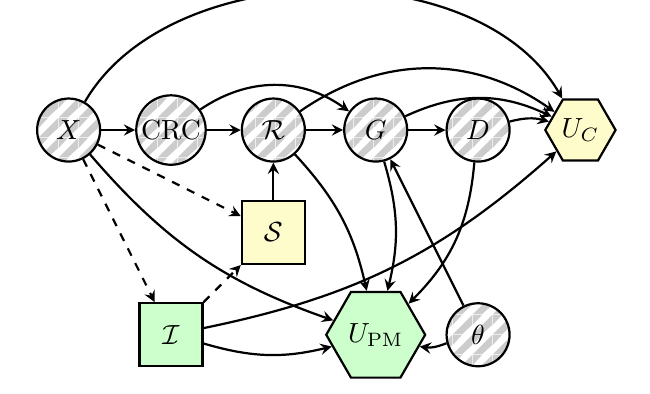
\begin{tikzpicture}[x=1.3cm, y=1.3cm]
            \useasboundingbox (-0.4, -1.3) rectangle (5.4, 2.0);
            
            % Nodes
            \node (ev)       at (0, 1)   [chance] {$X$};
            \node (crc)      at (1, 1)   [chance] {CRC};
            \node (res_scr)  at (2, 1)   [chance] {$\mathcal{R}$};
            \node (stage)    at (3, 1)   [chance] {$G$};
            \node (death)    at (4, 1)   [chance] {$D$};
            \node (util_cit) at (5, 1)   [utilityC] {$U_{C}$};
            \node (scr)      at (2, 0)   [decisionC] {$\mathcal{S}$};
            \node (I)        at (1, -1)  [decisionPM] {$\mathcal{I}$};
            \node (util_pm)  at (3, -1)  [utilityPM] {$U_{\text{PM}}$};
            \node (theta)    at (4, -1)  [chance] {$\theta$};

            % Disease and detection
            \draw [arrow] (ev) -- (crc);
            \draw [arrow] (crc) -- (res_scr);
            \draw [arrow] (scr) -- (res_scr);
            \draw [arrow, bend left=35] (crc) to (stage); 
            \draw [arrow] (res_scr) -- (stage);
            \draw [arrow] (stage) -- (death);
            
            % Information
            \draw [arrow, dashed] (ev) -- (I);
            \draw [arrow, dashed] (ev) -- (scr); 
            \draw [arrow, dashed] (I) -- (scr);

            % Into U_C (All Curved)
            \draw [arrow] (ev) to[out=60, in=120, looseness=0.9] (util_cit);
            \draw [arrow, bend left=35] (res_scr) to (util_cit); 
            \draw [arrow, bend left=25] (stage) to (util_cit);   
            \draw [arrow, bend left=15] (death) to (util_cit);
            \draw [arrow, bend right=15] (I) to (util_cit); 

            % Into U_PM (All Curved)
            \draw [arrow, bend right=15] (ev) to (util_pm); 
            \draw [arrow, bend left=15] (res_scr) to (util_pm); 
            \draw [arrow, bend left=15] (stage) to (util_pm);
            \draw [arrow, bend left=20] (death) to (util_pm);
            \draw [arrow, bend right=15] (I) to (util_pm);
            \draw [arrow, bend left=15] (theta) to (util_pm);
            
            \draw [arrow] (theta) -- (stage); % standard arc
        \end{tikzpicture}}
        \caption{CRC screening incentive problem}
        \label{fig:original_problem}
    \end{subfigure}
    \hfill
    % -----------------------------------------------------------
    % 2) PM'S PERSPECTIVE
    % -----------------------------------------------------------
    \begin{subfigure}[t]{0.32\textwidth}
        \centering
        \resizebox{\linewidth}{!}{%
        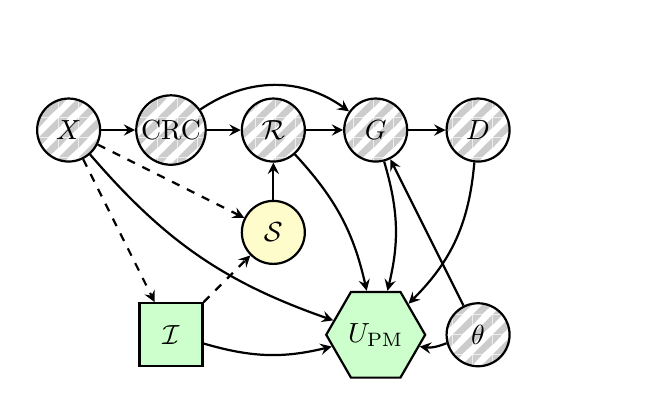
\begin{tikzpicture}[x=1.3cm, y=1.3cm]
            \useasboundingbox (-0.4, -1.3) rectangle (5.4, 2.0);
            
            \node (ev)       at (0, 1)   [chance] {$X$};
            \node (crc)      at (1, 1)   [chance] {CRC};
            \node (res_scr)  at (2, 1)   [chance] {$\mathcal{R}$};
            \node (stage)    at (3, 1)   [chance] {$G$};
            \node (death)    at (4, 1)   [chance] {$D$};
            \node (scr)      at (2, 0)   [chanceA] {$\mathcal{S}$};
            \node (I)        at (1, -1)  [decisionPM] {$\mathcal{I}$};
            \node (util_pm)  at (3, -1)  [utilityPM] {$U_{\text{PM}}$};
            \node (theta)    at (4, -1)  [chance] {$\theta$};

            \draw [arrow] (ev) -- (crc);
            \draw [arrow] (crc) -- (res_scr);
            \draw [arrow] (scr) -- (res_scr);
            \draw [arrow, bend left=35] (crc) to (stage);
            \draw [arrow] (res_scr) -- (stage);
            \draw [arrow] (stage) -- (death);
            
            \draw [arrow, dashed] (ev) -- (I);
            \draw [arrow, dashed] (ev) -- (scr);
            \draw [arrow, dashed] (I) -- (scr);

            % Into U_PM (All Curved)
            \draw [arrow, bend right=15] (ev) to (util_pm);
            \draw [arrow, bend left=15] (res_scr) to (util_pm);
            \draw [arrow, bend left=15] (stage) to (util_pm);
            \draw [arrow, bend left=20] (death) to (util_pm);
            \draw [arrow, bend right=15] (I) to (util_pm);
            \draw [arrow, bend left=15] (theta) to (util_pm);
            
            \draw [arrow] (theta) -- (stage);
        \end{tikzpicture}}
        \caption{PM's incentive problem}
        \label{fig:PM_problem}
    \end{subfigure}
    \hfill
    % -----------------------------------------------------------
    % 3) CITIZEN'S PERSPECTIVE
    % -----------------------------------------------------------
    \begin{subfigure}[t]{0.32\textwidth}
        \centering
        \resizebox{\linewidth}{!}{%
        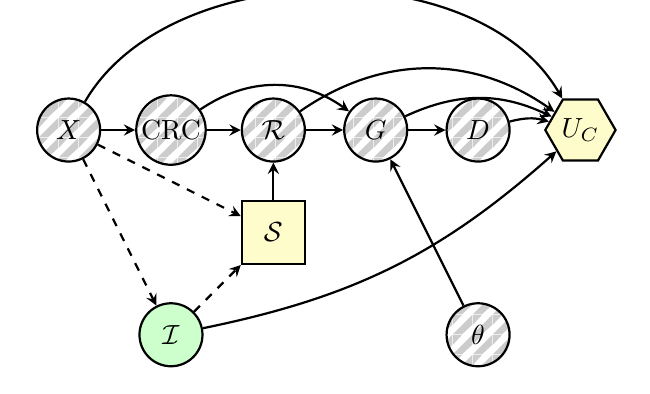
\begin{tikzpicture}[x=1.3cm, y=1.3cm]
            \useasboundingbox (-0.4, -1.3) rectangle (5.4, 2.0);
            
            \node (ev)       at (0, 1)   [chance] {$X$};
            \node (crc)      at (1, 1)   [chance] {CRC};
            \node (res_scr)  at (2, 1)   [chance] {$\mathcal{R}$};
            \node (stage)    at (3, 1)   [chance] {$G$};
            \node (death)    at (4, 1)   [chance] {$D$};
            \node (util_cit) at (5, 1)   [utilityC] {$U_{C}$};
            \node (scr)      at (2, 0)   [decisionC] {$\mathcal{S}$};
            \node (I)        at (1, -1)  [chanceD] {$\mathcal{I}$};
            \node (theta)    at (4, -1)  [chance] {$\theta$};

            \draw [arrow] (ev) -- (crc);
            \draw [arrow] (crc) -- (res_scr);
            \draw [arrow] (scr) -- (res_scr);
            \draw [arrow, bend left=35] (crc) to (stage);
            \draw [arrow] (res_scr) -- (stage);
            \draw [arrow] (stage) -- (death);
            
            \draw [arrow, dashed] (ev) -- (I);
            \draw [arrow, dashed] (ev) -- (scr);
            \draw [arrow, dashed] (I) -- (scr);

            % Into U_C (All Curved)
            \draw [arrow] (ev) to[out=60, in=120, looseness=0.9] (util_cit);
            \draw [arrow, bend left=35] (res_scr) to (util_cit);
            \draw [arrow, bend left=25] (stage) to (util_cit);
            \draw [arrow, bend left=15] (death) to (util_cit);
            \draw [arrow, bend right=15] (I) to (util_cit);
            
            \draw [arrow] (theta) -- (stage);
        \end{tikzpicture}}
        \caption{C's incentive problem}
        \label{fig:citizen_problem}
    \end{subfigure}

    \caption{BAIDs for the single citizen public scheme.}
    \label{fig:both_problems}
\end{figure*}


%%%%%%%%%%%%%%%%%%%%%%%%%%%%%%%%%%%%%
\subsubsection{Incentivising a single citizen}\label{sec:single_patient}
Let us first show how the PM sets the incentive for a single citizen with ARA, the basis for the incentive population schemes that follow.
 %%%%%%%%%%%%%%%%%%%%%%%%%%%%%%%%%%%%%
\subparagraph{PM problem.} The PM solves the decision analysis problem in Figure \ref{fig:PM_problem} by modelling C's screening decision with uncertainty $\pi_{PM}(s \mid \mathcal{I}, x)$, and also having probabilities about outcomes, $p_{PM}(c,r,g,d,\theta \mid s, \mathcal{I}, x)$, and their own utility function $u_{PM}(r,g,d,\mathcal{I},x, \theta)$. Given these, the PM's optimal incentive $\mathcal{I}^*(x)$ for a person with features $x$ is obtained as a solution to the maximum expected utility problem $\mathcal{I}^* (x)  =  \arg \max_{\mathcal{I}} \psi_{PM}(\mathcal{I} \mid x)$, where
\begin{align} \label{eq:max_util_PM}
  \psi_{PM}(\mathcal{I} \mid x) = & \quad \mathbb{E}_{\pi_{PM}(s \mid \mathcal{I}, x),\, p_{PM}(c,r,g,d,\theta \mid s, \mathcal{I}, x)} \big[u_{PM}(r,g,d,\mathcal{I},x, \theta)\big] \\
     = & \int \sum_{s} \sum_{r} \sum_{c} \sum_{g} \sum_{d} u_{PM}(r,g,d,\mathcal{I},x, \theta) \times \notag \\
    & \quad \times p_{PM}(c \mid x)\, p_{PM}(r \mid c,s)\, p_{PM}(g \mid c,r,\theta)\, p_{PM}(d \mid g)\, \pi_{PM}(s \mid \mathcal{I},x)\, p_{PM}(\theta) \, d\theta, \notag
\end{align}
possibly subject to constraints such as a maximum budget or a cap on the incentive to individuals. Except for $\pi_{PM}(s \mid \mathcal{I}, x)$, the ingredients in (\ref{eq:max_util_PM}) are standard in decision analysis terms \citep{french} (e.g. utility $u_{\text{PM}}$),  have been previously characterised (e.g. $p_{PM}(c \mid x)$ and $p_{PM}(r \mid c,s,scr)$ in \cite{corrales2024colorectal, corrales2025decision}), or will be described in the following sections ($p_{PM}(g \mid c,r,\theta)$, $p_{PM}(d \mid g)$ and $p_{PM}(\theta)$ in Section~\ref{sec:common_framework}). The remaining probability distribution $\pi_{PM}(s \mid \mathcal{I}, x)$ entails strategic thinking aspects that we now address, as it involves modelling C's problem from the perspective of the PM.

%%%%%%%%%%%%%%%%%%%%%%%%%%%%%%%%%%%
\subparagraph{Citizen's problem.} To assess such distribution, consider $C$'s problem (Figure \ref{fig:citizen_problem}) for a given $\mathcal{I}$ and $x$. Since the PM does not fully know $C$'s beliefs $p_C$ and preferences $u_C$, the solution requires modelling the PM's uncertainty about the citizen's utility and probability distributions $(u_{C}, p_{C})$ through a random utility $U_C$ and a random distribution $P_C$ \citep{rios2009adversarial}, represented as $ F_C  \sim ( U_C, P_C )$. We call a single draw from $F_C$ a citizen \emph{type} $t$ \citep{assaf2020bayesian}. Across a population, $F_C$ describes how citizens with the same $x$ differ, and types are independent draws from it. This induces a distribution over the citizens' expected utility, defined through 
\begin{align}\label{eq:randexp}
    \Psi_C (s \mid \mathcal{I} , x) = & \quad \mathbb{E}_{P_{C}(c,r,g,d,\theta \mid s, x)} \big[U_C(r,g,d,\mathcal{I},x, \theta) \big]  \\
    = & \int \sum_{r} \sum_{c} \sum_{g} \sum_{d} U_C(r,g,d, \mathcal{I},x,\theta) \times \nonumber \\
     & \qquad  \times \, P_C(c \mid x)\, P_C(r \mid c,s)\, P_C(g \mid c,r,\theta)\, P_C(d \mid g)\, P_C(\theta) \, d\theta. \nonumber
\end{align}
The PM then estimates the required probabilities through
\begin{align}\label{eq:probPM}
    \pi_{PM}(s \mid \mathcal{I}, x) = \mathbb{P}_{F_C}\big[\arg \max_{s' \in \{0,1\}} \Psi_C (s' \mid \mathcal{I} , x) = s\big].
\end{align}
Computationally, $\pi_{PM}$ is estimated by Monte Carlo, by drawing $N_C$ types from $F_C$, the citizen's problem is solved under each, and the share of draws in which $s$ is optimal estimates $\pi_{PM}(s \mid \mathcal{I}, x)$, as summarised in Appendix~\ref{app:simulation_public_forecast}. These probabilities are then input into \eqref{eq:max_util_PM} to determine $\mathcal{I}^*(x)$.



%%%%%%%%%%%%%%%%%%%%%%%%%%%%%%%%%%%%%%%%%%%%%
\subsubsection{Incentivising the entire population}\label{sec:incent}

\begin{figure}[h!]
    \centering
    \resizebox{0.45\linewidth}{!}{%
    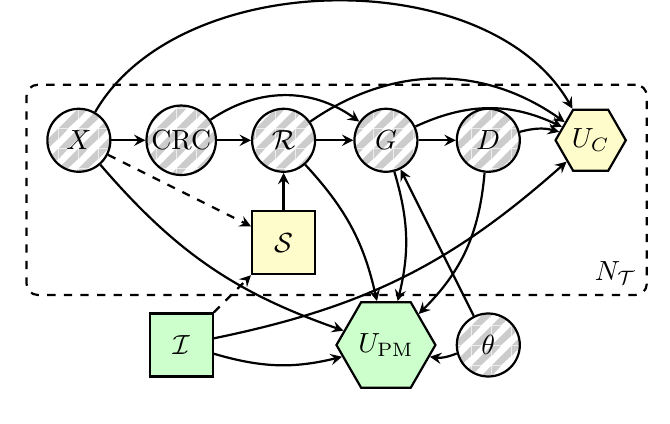
\begin{tikzpicture}[x=1.3cm, y=1.3cm]
        \useasboundingbox (-0.5, -1.5) rectangle (5.5, 2.1);
        
        % 1. CITIZEN LAYER (inside the plate)
        \node (ev)       at (0, 1)   [chance] {$X$};
        \node (crc)      at (1, 1)   [chance] {CRC};
        \node (res_scr)  at (2, 1)   [chance] {$\mathcal{R}$};
        \node (stage)    at (3, 1)   [chance] {$G$};
        \node (death)    at (4, 1)   [chance] {$D$};
        \node (util_cit) at (5, 1)   [utilityC] {$U_{C}$};
        \node (scr)      at (2, 0)   [decisionC] {$\mathcal{S}$};
        
        % 2. COMMON TO THE POPULATION (outside the plate)
        \node (I)        at (1, -1)  [decisionPM] {$\mathcal{I}$};
        \node (util_pm)  at (3, -1)  [utilityPM] {$U_{\text{PM}}$};
        \node (theta)    at (4, -1)  [chance] {$\theta$};
        
        % 3. THE PLATE
        \begin{scope}[on background layer]
            \node [draw, thick, rectangle, rounded corners, dashed,
                   fit=(ev) (crc) (util_cit) (scr),
                   inner sep=0.25cm,
                   label={[anchor=south east, inner sep=4pt]south east:$N_{\mathcal{T}}$}] (plate) {};
        \end{scope}
        
        % 4. ARROWS inside the plate
        \draw [arrow] (ev) -- (crc);
        \draw [arrow, dashed] (ev) -- (scr);
        \draw [arrow] (crc) -- (res_scr);
        \draw [arrow] (scr) -- (res_scr);
        \draw [arrow, bend left=35] (crc) to (stage);
        \draw [arrow] (res_scr) -- (stage);
        \draw [arrow] (stage) -- (death);
        
        % Into U_C (All curved)
        \draw [arrow] (ev) to[out=60, in=120, looseness=0.9] (util_cit);
        \draw [arrow, bend left=35] (res_scr) to (util_cit);
        \draw [arrow, bend left=25] (stage) to (util_cit);
        \draw [arrow, bend left=15] (death) to (util_cit);
        
        % 5. ARROWS crossing the plate into U_PM (All Curved)
        \draw [arrow, bend right=15] (ev) to (util_pm);
        \draw [arrow, bend left=15] (res_scr) to (util_pm);
        \draw [arrow, bend left=15] (stage) to (util_pm);
        \draw [arrow, bend left=20] (death) to (util_pm);
        
        % 6. ARROWS from the common nodes
        \draw [arrow, dashed] (I) -- (scr);
        \draw [arrow] (theta) -- (stage);
        
        % From common nodes to utilities (All curved)
        \draw [arrow, bend right=15] (I) to (util_cit);
        \draw [arrow, bend right=15] (I) to (util_pm);
        \draw [arrow, bend left=15] (theta) to (util_pm);
    \end{tikzpicture}}
    \caption{Incentivising the entire population with a common incentive.}
    \label{fig:common_incentive_problem}
\end{figure}

Most currently active public programmes are designed so that the incentive is common for all citizens within the target population \citep{facciorusso2021addition}. Let the $N_{\mathcal{T}}$ citizens of the target population $\mathcal{T}$ have covariates $\mathbf{x} = (x_i)_{i=1}^{N_\mathcal{T}}$, and designate with $\mathbf{s}, \mathbf{c}, \mathbf{r}, \mathbf{g}, \mathbf{d}$ the corresponding vectors of decisions, CRC statuses, results, stages, and CRC deaths. The PM now seeks $\mathcal{I}^{*} = \arg \max_{\mathcal{I}} \psi_{PM}(\mathcal{I} \mid \mathcal{T})$, where
\begin{align}\label{eq:expected_util_population}
 \psi_{PM}&(\mathcal{I} \mid \mathcal{T})
  = \mathbb{E}_{\pi_{PM}(\mathbf{s} \mid \mathcal{I}, \mathcal{T}),\, p_{PM}(\mathbf{c}, \mathbf{r}, \mathbf{g}, \mathbf{d}, \theta \mid \mathbf{s}, \mathcal{I}, \mathcal{T})} \big[u_{PM}( \mathbf{r}, \mathbf{g}, \mathbf{d}, \mathcal{I}, \mathbf{x}, \theta)\big] \\
  & \qquad \ \ = \int   p_{PM}(\theta)\, \bigg[ \sum_{\mathbf{s}} \sum_{\mathbf{r}} \sum_{\mathbf{c}} \sum_{\mathbf{g}} \sum_{\mathbf{d}}
     u_{PM}\big( \mathbf{r}, \mathbf{g}, \mathbf{d}, \mathcal{I}, \mathbf{x}, \theta \big) \times \notag\\
  &\quad  \times
     \prod_{i=1}^{N_{\mathcal{T}}}
        p_{PM}(c_i\mid x_i)\, p_{PM}(r_i\mid c_i, s_i)\, p_{PM}(g_i \mid c_i, r_i, \theta)\, p_{PM}(d_i \mid g_i)\, \pi_{PM}(s_i\mid\mathcal{I}, x_i) \bigg]\, d\theta. \notag
\end{align}
As seen in Figure \ref{fig:common_incentive_problem}, we now cover a set of citizens. The sums in \eqref{eq:expected_util_population} run over a space growing exponentially in $N_{\mathcal{T}}$. Note that $\theta$ lies outside the product as, given $\theta$, citizens are independent, but $\theta$ itself is shared by all of them. For a general utility $u_{\text{PM}}$, the expectation must be taken by simulation. A value $\theta \sim p_{PM}(\theta)$ is drawn; replicates of the entire population outcome are then drawn given it, with $c_i \sim p_{PM}(c \mid x_i)$, $s_i \sim \pi_{PM}(s \mid \mathcal{I}, x_i)$, $r_i \sim p(r \mid c_i, s_i)$, $g_i \sim p(g \mid c_i, r_i, \theta)$ and $d_i \sim p(d \mid g_i)$ for each citizen; $u_{\text{PM}}$ is evaluated once per replicate and averaged over replicates and draws of $\theta$. Simulation schemes are detailed in Appendix~\ref{app:simulation_public}.

Every replicate requires $\pi_{PM}(s \mid \mathcal{I}, x_i)$, and hence a solution of the citizen's problem, for every incentive and citizen. Citizens who share the covariates on which that problem depends share this probability, so it is computed once per covariate profile. The PM's expected utility is estimated on a grid $\mathcal{G}_{\mathcal{I}}$ of incentives, and $\mathcal{I}^*$ is read from a surrogate $\widehat{\psi}_{PM}(\mathcal{I})$ fitted to the estimates $\{(\mathcal{I}_k, \psi_{PM}(\mathcal{I}_k \mid \mathcal{T}))\}_{k=1}^{|\mathcal{G}_{\mathcal{I}}|}$, e.g.\ a Gaussian process \citep{gramacy2020surrogates}. Common random numbers (CRN)  are used across the incentive grid and across draws of $\theta$ to reduce the variance of simulation experiments \citep{law1991simulation}.


 
%%%%%%%%%%%%%
\subsection{Outcome based payments}\label{sec:OBP}
Governments increasingly partner with private providers to deliver public services, seeking the flexibility, capacity and expertise they lack, and sharing with the provider the risk of the service falling short \citep{roehrich2014public}. The private-public scheme studied here is \emph{outcome-based payments (OBP)}, described in detail in \cite{vlaanderen2019design} and \cite{fox2021evaluating}. In these financial models, payment is tied to the outcomes achieved rather than to the mere delivery of a service or product. One example in the healthcare sector is the {\em Best Practice Tariffs} model of the English NHS \citep{kristensen2016optimal}.

In this type of scheme, besides the agents PM and C, a third actor emerges: a service provider (SP) which delivers screening on behalf of the PM. Delegation is attractive because the SP can do what a centrally run programme cannot, such as varying incentives across population groups, contact non-responders in person, and help them take and return the test. That same capacity is, however, effort that the PM cannot observe so the PM pays for observable outcomes instead. Thus, the OBP scheme thus reimburses the SP conditionally on meeting predefined screening and detection targets.\footnote{An independent auditor verifies the reported outcomes. Its role is what renders those outcomes contractible in the first place, but it is passive as regards incentive design, and we leave it, and its cost, outside the model.}

OBPs may adopt numerous parametric forms. To fix the discussion, we use one comprising a payment for the care delivered and two further payments conditional on what the campaign achieves. The SP receives from the PM the aggregation of
\begin{itemize}
    \item {\em Base payment} (BP). Reimbursement, at the PM's unit prices, of the care delivered. This includes the tests implemented and the confirmatory colonoscopies performed.
    \item {\em Outcome payment}. An amount of up to $z_4$ € per invited citizen, earned as coverage rises from a lower threshold $z_2$ to an upper threshold $z_1$. Nothing is earned when less than a fraction $z_2$ of the target population is screened, the full amount is earned at or above $z_1$, and a proportional share is earned in between.
    \item \rev{{\em Completion payment}. An additional payment of $z_3$ € per follow-up colonoscopy completed after a positive screening test.}\revdel{{\em Bonus}. An additional payment of $z_3$ € per CRC case confirmed through the screening pathway.}
\end{itemize}
Let us write $\mathcal{O}$ for the audited screening record of the campaign, from which follow the cost $BP(\mathcal{O})$ of the care delivered, the fraction $q(\mathcal{O})$ of the target population screened, and the number $n(\mathcal{O})$ of \rev{follow-up colonoscopies completed}\revdel{CRC cases confirmed}. The contract then pays
\begin{align}\label{eq:obp}
  obp(\mathcal{O}, z) &= BP(\mathcal{O}) + z_4 \cdot N_{\mathcal{T}} \cdot \omega\big(q(\mathcal{O}); z_1, z_2\big) + z_3 \cdot n(\mathcal{O}),
\end{align}
where the share of the outcome payment earned at coverage $q$ is
\begin{align}\label{eq:omega}
  \omega(q; z_1, z_2) =
  \begin{cases}
    0, & q \leq z_2, \\[2pt]
    \dfrac{q - z_2}{z_1 - z_2}, & z_2 < q < z_1, \\[8pt]
    1, & q \geq z_1,
  \end{cases}
\end{align}
and $z = (z_1, z_2, z_3, z_4)$ lies in $Z = \{ z : 0 \leq z_2 < z_1 \leq 1,\ z_3 \geq 0,\ z_4 \geq 0 \}$. The outcome payment has the shape of the \emph{Quality and Outcomes Framework} \citep{campbell2009effects}, a price per point scaled by list size and by achievement between two thresholds.


Observe that the three payments focus on three distinct events: test delivered, population covered, and \rev{diagnosis completed}\revdel{cases confirmed}. BP reimburses the care delivered, but neither the invitations nor the incentives nor any other effort of the SP is reimbursed; these are financed from the outcome payment and the \rev{completion payment}\revdel{bonus}, which is what makes the contract outcome-based. Coverage is measured against the whole target population rather than against those approached, so a threshold cannot be met by approaching fewer citizens. The four $z$ parameters separate both roles a contract must fill: $z_1$ and $z_2$ fix the coverage over which the outcome payment is earned, while $z_4$ and $z_3$ fix what the PM pays for coverage and per \rev{diagnosis completed}\revdel{case confirmed}. \rev{The completion payment is paid on volume, one event at a time, while the outcome payment depends on whether coverage crosses its thresholds; Section~\ref{sec:obp_scheme_results} shows that the former is what makes the contract robust to the SP's attitude to risk. Paying per confirmed cancer instead is worth the same to the PM (Table~\ref{tab:obp_sensitivity}), but it pays on about seventeen times fewer events, and completion is a process measure, available within weeks, of the kind proposed for HEDIS \citep{buist2026}.}



%%%%%%%%%%%%%%%%%
\subsubsection{Modelling OBPs through a multi-agent influence diagram}
The proposed OBP scheme adopts the MAID structure in Figure~\ref{fig:multiagent_obp}. Blue nodes refer to the SP, with green and yellow denoting PM and C, respectively, as in the public scheme. Citizen nodes are those in Figure~\ref{fig:common_incentive_problem}.

\begin{figure}[h!]
    \centering
    \resizebox{0.65\linewidth}{!}{%
    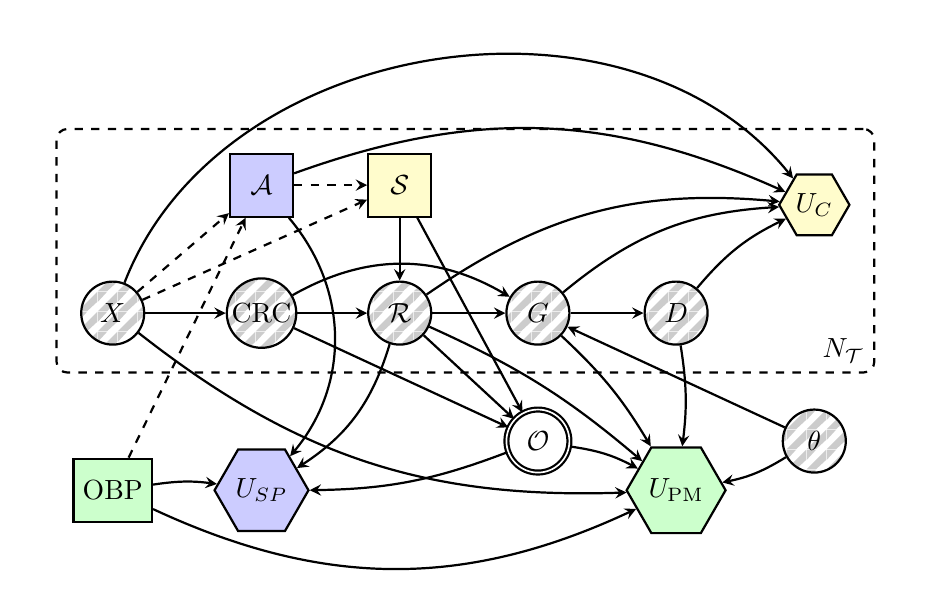
\begin{tikzpicture}[x=1.35cm, y=1.25cm]
        \useasboundingbox (-0.8, -2.4) rectangle (7.4, 3.2);
        % 1. DECISIONS (top), CITIZEN CHAIN (middle)
        \node (ev)       at (0, 0.3)     [chance]     {$X$};
        \node (A)        at (1.4, 1.6)   [decisionSP] {$\mathcal{A}$};
        \node (scr)      at (2.7, 1.6)   [decisionC]  {$\mathcal{S}$};
        \node (crc)      at (1.4, 0.3)   [chance]     {CRC};
        \node (res_scr)  at (2.7, 0.3)   [chance]     {$\mathcal{R}$};
        \node (stage)    at (4.0, 0.3)   [chance]     {$G$};
        \node (death)    at (5.3, 0.3)   [chance]     {$D$};
        \node (util_cit) at (6.6, 1.4)   [utilityC]   {$U_{C}$};
        % 2. COMMON NODES (outside the plate)
        \node (theta)    at (6.6, -1)  [chance]     {$\theta$};
        \node (detected) at (4.0, -1)  [determ]     {$\mathcal{O}$};
        \node (OBP)      at (0, -1.5)    [decisionPM] {OBP};
        \node (util_sp)  at (1.4, -1.5)  [utilitySP]  {$U_{SP}$};
        \node (util_pm)  at (5.3, -1.5)  [utilityPM]  {$U_{\text{PM}}$};
        % 3. THE PLATE
        \begin{scope}[on background layer]
            \node [draw, thick, rectangle, rounded corners, dashed,
                   fit=(ev) (A) (scr) (crc) (util_cit),
                   inner sep=0.3cm,
                   label={[anchor=south east, inner sep=4pt]south east:$N_{\mathcal{T}}$}] (plate) {};
        \end{scope}
        % 4. CHANCE ARCS (straight)
        \draw [arrow] (ev) -- (crc);
        \draw [arrow] (crc) -- (res_scr);
        \draw [arrow] (scr) -- (res_scr);
        \draw [arrow, bend left=30] (crc) to (stage);
        \draw [arrow] (res_scr) -- (stage);
        \draw [arrow] (stage) -- (death);
        \draw [arrow] (theta) -- (stage);
        % 5. INFORMATION ARCS (dashed, into decisions)
        \draw [arrow, dashed] (ev) -- (A);
        \draw [arrow, dashed] (ev) -- (scr);
        \draw [arrow, dashed] (A) -- (scr);
        \draw [arrow, dashed] (OBP) -- (A);
        % 6. AUDITED RECORD (straight, into a deterministic node)
        \draw [arrow] (crc) -- (detected);
        \draw [arrow] (scr) -- (detected);
        \draw [arrow] (res_scr) -- (detected);
        % 7. VALUE ARCS (curved, into utilities)
        \draw [arrow, bend left=12] (death) to (util_cit);
        \draw [arrow, bend left=18] (stage) to (util_cit);
        \draw [arrow, bend left=20] (res_scr) to (util_cit);
        \draw [arrow, bend left=22] (A) to (util_cit);
        \draw [arrow, bend left=60] (ev) to (util_cit);
        \draw [arrow, bend left=40] (A) to (util_sp);
        \draw [arrow, bend left=20] (res_scr) to (util_sp);
        \draw [arrow, bend left=10] (detected) to (util_sp);
        \draw [arrow, bend left=8]  (OBP) to (util_sp);
        \draw [arrow, bend right=25] (OBP) to (util_pm);
        \draw [arrow, bend right=20] (ev) to (util_pm);
        \draw [arrow, bend left=8]  (res_scr) to (util_pm);
        \draw [arrow, bend left=8]  (stage) to (util_pm);
        \draw [arrow, bend left=8]  (death) to (util_pm);
        \draw [arrow, bend left=10] (detected) to (util_pm);
        \draw [arrow, bend left=10] (theta) to (util_pm);
    \end{tikzpicture}}
    \caption{MAID for the OBP scheme. The dashed plate replicates the citizen subproblem over $N_{\mathcal{T}}$ citizens of the target population; $\theta$, the OBP contract, audited record $\mathcal{O}$ and value nodes of the PM and the SP lie outside it.}
    \label{fig:multiagent_obp}
\end{figure}
Every citizen in $\mathcal{T}$ receives the
programme's standard invitation as in the public scheme, as organised programmes must invite their whole eligible population. On top of it, the SP has \rev{four}\revdel{three} operational levers, summarised in decision node $\mathcal{A}$:
\begin{itemize}
    \item an \emph{incentive} $\mathcal{I} \geq 0$, paid to the citizen upon completing screening, possibly differing across citizens;
  \item \emph{navigation support}, $\ell^{N} \in \{0,1\}$: a personal contact with a citizen who has not responded, explaining their risk and the purpose of the test. It acts on what the citizen believes, aimed at correcting the under-perception of their own risk;
  \item \emph{access support}, $\ell^{A} \in \{0,1\}$: practical help for a citizen who has not responded to obtain and return the test, such as a nearby pick-up point or home collection. It acts on what participation costs the citizen, lowering the burden of the test\rev{;}\revdel{.}
  \rev{\item \emph{follow-up navigation}, $\ell^{F} \in \{0,1\}$: a personal contact with a citizen who tested positive and has not booked the confirmatory colonoscopy. It acts on the completion of the diagnosis rather than on participation.}
\end{itemize}
The offer to a citizen is therefore $a = (\mathcal{I}, \ell)$, with $\ell = (\ell^{N}, \ell^{A}\rev{, \ell^{F}})$, so $a \in \mathbb{R}_{+} \times \{0,1\}^{\rev{3}}$\revdel{$\{0,1\}^2$}. The SP does not observe citizen types, so the offer to citizen $i$ can depend on them only through their known covariates, $a_i = a(x_i)$. The \emph{incentive campaign} is the rule $\mathbf{a} = (a(x_i))_{i \in \mathcal{T}}$, fixed before invitations are sent.

Support is offered only to citizens who do not respond to the invitation, who
then decide again with the same incentive. The PM observes neither
$\mathbf{a}$ nor who was supported, only the record $\mathcal{O}$. Decision-making hence proceeds as follows:
\begin{itemize}
    \item The PM designs the scheme, in our case fixing $z$, by modelling how the SP will run the campaign and how citizens will respond to it.

    \item The SP, observing $z$, fixes its campaign, modelling how citizens will react to it.

    \item Citizens are asked to decide whether to participate or not. Those who accept are assumed to complete the programme, and the incentive is paid. A positive result calls for a confirmatory colonoscopy, which establishes the citizen's CRC status and enters them into the corresponding care pathway\rev{; a share of positive citizens do not complete it, which follow-up navigation may reduce}. Those who do not respond may receive navigation or access support under the SP's plan and decide again.

    \item Outcomes are audited through $\mathcal{O}$ and the PM pays the SP according to $obp(\mathcal{O}, z)$.

\end{itemize}

The record node $\mathcal{O}$ collects the number of citizens screened, the number of positive screening results, \rev{the number of follow-up colonoscopies completed, }the number of CRC cases confirmed after colonoscopy, and the cost of the care delivered. These are the outcomes required by the PM to assess the contract in \eqref{eq:obp}.

The rounded box in the MAID denotes replication of the citizen problem over the $N_{\mathcal{T}}$ individuals of the target population. It does not, however, mean independence, as $\mathcal{O}$ aggregates all citizens' subproblems. Hence the coverage thresholds are evaluated jointly on the whole target population, and the SP values its global position rather than each citizen separately. Therefore, its optimisation does not decompose across individuals, in contrast to the per-citizen treatment of Section~\ref{sec:single_patient}. 




%%%%%%%%%%%%%%%%%%%%%%%%%
\subsubsection{Solution approach}\label{sec:OBP_inc}
Similar to the public scheme, the PM requires modelling the other agents' problems to find its optimal contract design. 
\subparagraph{Citizen's problem.}
It is similar to that in Section~\ref{sec:single_patient}, with the offer now
made by the SP. The SP must forecast the response, so it holds its own random model of the
citizen, which need not coincide with the PM's and which we also write
$F_C \sim (U_C, P_C)$. It yields, for a citizen with covariates $x$ offered
$a = (\mathcal{I}, \ell)$,
\begin{align} \label{eq:psi_C}
    \Psi_C(s \mid a, x)
    &= \mathbb{E}_{P_C(c \mid a, x)\, P_C(r \mid c, s)\,
        P_C(g \mid c, r, \theta)\, P_C(d \mid g)\, P_C(\theta)}
       \big[ U_C( r, g, d, a, x, \theta ) \big]  \\
    &= \int \sum_{c,r,g,d}
       U_C( r, g, d, a, x, \theta )\,
       P_C(c \mid a, x)\, P_C(r \mid c, s)\,
       P_C(g \mid c, r, \theta)\, P_C(d \mid g)\, P_C(\theta) \,
       \mathrm{d}\theta. \notag
\end{align}
The campaign reaches the citizen through three channels: the incentive enters
their payoff, as in the public scheme; navigation acts on $P_C(c \mid a, x)$,
their assessment of their own risk; and access support acts on $U_C$ through
the burden of the test. The SP's forecast of acceptance is then
\begin{align} \label{eq:p_s}
    \pi_{SP}(s \mid a, x) = \mathbb{P}_{F_C}\!\left[
    \arg\max_{s'} \Psi_C(s' \mid a, x) = s \right].
\end{align}

%%%%%%%%%%%%%%%%%%%%%%%%%%%%%%%%%%%%%%%%%%%%%%%
\subparagraph{SP problem.}
Observing the contract $z$, the SP chooses a campaign $\mathbf{a}$ from the set
$\mathbb{A}$ of those available to it, which includes declining the contract.
It evaluates its global position under a utility $u_{SP}$, so its objective is
\begin{align}\label{eq:sp_util}
  \psi_{SP}(\mathbf{a} \mid z, \mathcal{T})
  &= \mathbb{E}_{\pi_{SP}(\mathbf{s} \mid \mathbf{a}, \mathcal{T})\,
     p_{SP}(\mathbf{c}, \mathbf{r} \mid \mathbf{s}, \mathcal{T})}
     \big[ u_{SP}( \mathbf{a}, \mathbf{s}, \mathbf{r}, \mathcal{O}, z ) \big] \\
  &= \sum_{\mathbf{s}} \sum_{\mathbf{c}} \sum_{\mathbf{r}}
    u_{SP}( \mathbf{a}, \mathbf{s}, \mathbf{r}, \mathcal{O}, z )
    \prod_{i = 1}^{N_{\mathcal{T}}}
      p_{SP}(c_i \mid x_i)\, \pi_{SP}(s_i \mid a_i, x_i)\,
      p_{SP}(r_i \mid c_i, s_i), \notag
\end{align}
where $\mathcal{O}$ is determined by $(\mathbf{c}, \mathbf{r}, \mathbf{x})$.
The contract pays on counts, so neither $\theta$ nor the stage and survival of
citizens enter the SP's problem. The SP adopts the maximum expected
utility campaign,
\begin{align}\label{eq:sp_argmax}
  \mathbf{a}^{*} = \arg\max_{\mathbf{a} \in \mathbb{A}}
    \psi_{SP}(\mathbf{a} \mid z, \mathcal{T}).
\end{align}

The PM does not observe the SP's choice, and applies a second ARA step to it
through a random model $F_{SP} \sim (U_{SP}, P_{SP})$, where $U_{SP}$ carries
the PM's uncertainty about the SP's preferences and costs, and $P_{SP}$ its
beliefs, including the citizen model $F_C$ on which $\pi_{SP}$ rests. The SP's
objective is then a random function $\Psi_{SP}(\mathbf{a} \mid z, \mathcal{T})$
and its maximiser a random optimal campaign,
\begin{align}
  \mathbf{A}^{*}(z) = \arg\max_{\mathbf{a} \in \mathbb{A}}
    \Psi_{SP}(\mathbf{a} \mid z, \mathcal{T}),
\end{align}
assumed unique almost surely. The PM's forecast is its distribution,
\begin{align} \label{eq:sp_forecast}
    \pi_{PM}(B \mid z, \mathcal{T})
    = \mathbb{P}_{F_{SP}}\big[\, \mathbf{A}^{*}(z) \in B \,\big],
    \qquad B \subseteq \mathbb{A},
\end{align}
which reduces to
$\pi_{PM}(\mathbf{a} \mid z, \mathcal{T}) =
\mathbb{P}_{F_{SP}}[\mathbf{A}^{*}(z) = \mathbf{a}]$ when $\mathbb{A}$ is
finite.


\subparagraph{PM problem.}
The PM needs to choose the OBP scheme, which amounts to selecting the parameters $z$ based on its expected utility function
\begin{align}\label{eq:pm_util}
    \psi_{PM}(z \mid \mathcal{T}) &= \mathbb{E}_{\pi_{PM}(\mathbf{a} \mid z, \mathcal{T})\, \pi_{PM}(\mathbf{s} \mid \mathbf{a}, \mathbf{x})\, p_{PM}(\mathbf{c}, \mathbf{r}, \mathbf{g}, \mathbf{d}, \theta \mid \mathbf{s}, \mathbf{x})} \big[ u_{PM}( \mathbf{r}, \mathbf{g}, \mathbf{d}, \mathbf{x}, \theta, \mathcal{O}, z) \big] \\
    &  = \int p_{PM}(\theta) \int_{\mathbb{A}} \pi_{PM}(\mathrm{d}\mathbf{a} \mid z, \mathcal{T}) \bigg[ \sum_{\mathbf{s}} \sum_{\mathbf{r}} \sum_{\mathbf{c}} \sum_{\mathbf{g}} \sum_{\mathbf{d}}
     u_{PM}( \mathbf{r}, \mathbf{g}, \mathbf{d}, \mathbf{x}, \theta, \mathcal{O}, z) \times \nonumber \\
    & \ \times \prod_{i=1}^{N_{\mathcal{T}}} p_{PM}(c_i \mid x_i)\, p_{PM}(r_i \mid c_i, s_i)\, p_{PM}(g_i \mid c_i, r_i, \theta)\, p_{PM}(d_i \mid g_i)\, \pi_{PM}(s_i \mid a_i, x_i) \bigg]\,  \, d\theta. \notag
\end{align}
The PM's utility values the health outcomes and bears the contractual payment $obp(\mathcal{O}, z)$, with $\mathcal{O}$ determined by the realised outcomes. The SP's campaign enters only through the PM's forecast of citizen acceptance, $\pi_{PM}(\mathbf{s} \mid \mathbf{a}, \mathbf{x}) = \prod_i \pi_{PM}(s_i \mid a_i, x_i)$, which changes who accepts screening. Each factor is that of the public scheme with the offer $a_i$ in place of the incentive $\mathcal{I}$, the support entering the citizen's problem as in \eqref{eq:psi_C}. This does not need to coincide with the SP's forecast $\pi_{SP}(s_i \mid a_i, x_i)$, it does so only if the SP holds the PM's citizen model. The contract parameters act one step further back, through the forecast $\pi_{PM}(\cdot \mid z, \mathcal{T})$ of \eqref{eq:sp_forecast} over which the campaign is integrated, as the PM cannot choose the campaign but only the terms under which the SP chooses it and assessing that forecast is the PM's strategic step.


As in Section~\ref{sec:incent}, a general $u_{\text{PM}}$ does not let the expectation factorise, and the shared block of $\theta$ couples the citizens. Here, a further expectation over the SP's campaign sits on top. We therefore proceed by simulation, following the scheme in Appendix~\ref{app:simulation_OBP_utility}. Choosing a finite grid $\mathcal{G} \subset Z$, we estimate $\psi_{PM}(z \mid \mathcal{T})$ at each point and take the maximiser $z^{*}$.


%%%%%%%%%%%%%%%%%%%%%%%%%%%%%%%%%%%%%%%%%%%%
\section{Modelling and results} \label{sec:modelling_results}
We now specify the models of Section~\ref{sec:incentive_problem_definition} for the Spanish FIT based screening system and solve them to determine the most appropriate scheme. Section~\ref{sec:public_scheme_modelling} specifies the valuation of outcomes and the citizen and PM models shared by both schemes. Section~\ref{sec:public_scheme_results} solves the public scheme. Section~\ref{sec:obp_modelling} specifies and solves the outcome-based payment. Finally, Section~\ref{sec:comparison} compares the schemes. Parameters are taken from published sources when available; the remaining ones are stated as assumptions and assessed through sensitivity analyses. As a relevant note, the parametric models chosen here are instrumental and may be discussed or replaced in other case studys with different modelling needs and assumptions.

Both incentive schemes are evaluated on the records of the 2016 medical database described in Appendix \ref{app:models}, which covers $339{,}707$ Spanish citizens. Two policies select the target population $\mathcal{T}$ for screening, both involving the standard \emph{faecal immunochemical test} (FIT). The \emph{age-based} policy invites all $N_{\mathcal{T}} = 49{,}074$ citizens aged 60--69%, the oldest band of the 50--69 programmes run in Spain
. The \emph{risk-based} policy invites the same number of citizens with the highest $p_{PM}(c=1 \mid x)$, of whom 10{,}940 (22.3\%) are younger than 60. We refer to the age-based policy without incentive as the \emph{status quo}. For simplicity, we assume a single screening round and full adherence once a citizen accepts. Section~\ref{sec:conclusions} discusses the consequences of these and other structural assumptions.

The case study is a worked example rather than a straight recommendation for Spain. An authority using the procedure would replace its inputs with its own risk model, uptake, costs and valuation of health, and would obtain the optimal policy, the uncertainty around it, and the inputs on which the ranking of options depends. Here these are the response of participation to money and the effect and cost of access support, on which evidence, for instance from a pilot that randomises the incentive, should be gathered first.

%%%%%%%%%%%%%%%%%%%%%%%%%%%%%%%%%%%
\subsection{Model specification} \label{sec:public_scheme_modelling}
Assume the PM has access to a CRC risk model, such as the one sketched in Appendix \ref{app:models}, so they are accurately informed of the probabilities $p_{PM}(c \mid x)$. Citizens are assumed to hold their own, possibly distorted, risk assessment $p_C(c \mid x)$. Several literature reviews point to a lack of information and risk misconception as one of the main reasons for low participation in screening programmes; see, e.g., \cite{wee2005factors}, \cite{le2023exploring}, or \cite{berg2022reasons}. 
 
Specifically for the case of the database considered, the PM's $p_{PM}(c=1 \mid x)$ is given by a risk model evaluated on all the covariates available in the records, while the citizens' $p_{C}(c=1 \mid x)$ is given by a risk model evaluated only on a smaller subset of them, the variables that citizens read as risk factors. Concretely, it is assumed that the citizens do not read three medical conditions as risk factors, thus showing information imbalance with respect to the PM. The citizen model is calibrated on the age-based policy and held fixed across policies (Section~\ref{sec:citizen_model}), so uptake differs between them only because they invite different citizens. Section~\ref{sec:common_framework} specifies how outcomes are valued, and Sections~\ref{sec:citizen_model} and~\ref{sec:pm_model} describe the citizen and PM models. 

\subsubsection{Common framework}\label{sec:common_framework}
Common to both agents are the horizon over which health accrues and the health consequences of CRC and of screening, together with their uncertainty about them. 
\paragraph{Valuing health.} Assume that PM and C value health outcomes in monetary terms, pricing \emph{quality-adjusted life years} (QALYs) at the Spanish cost-effectiveness threshold of $v = 30{,}000$€ per QALY, consistent with Spanish Health Technology Assessment practice \citep{vallejo2018estimating, sacristan2002que}. Further, assume that a citizen with covariates $x$ has a \emph{remaining life expectancy} $\bar{Y}(x)$, and each of those life-years is quality-adjusted through the EQ-5D \emph{quality-of-life} weight $h(x)$, with $h$ on a scale from 0 (death) to 1 (full health) \citep{garcia2016normative} (Table \ref{tab:age_stratified}). These weights describe health states and the agents' preferences enter only through their utilities over the resulting monetary values. Health accrues as a stream over the years a citizen survives, and we write $\mathrm{PV}(Y,\lambda) = \big(1-(1+\lambda)^{-Y}\big)/\lambda$ for the present value at rate $\lambda$ of one unit per year over $Y$ years. Each agent applies its own rate. The PM discounts health at the social rate $\lambda_{PM} = 0.03$, a convention in Spanish Health Technology Assessment (HTA) \citep{lopez2010spanish}, and citizens do so at their own $\lambda_C$, which is generally larger, thus under-appreciating future consequences.


\paragraph{CRC stage and survival.} We assume that a citizen without CRC survives the whole horizon, $Y = \bar Y(x)$. For a citizen with CRC, what screening changes is the stage $g$ at which the cancer is diagnosed. A cancer detected by screening ($r=1$) has distribution $\boldsymbol{\phi}^{\text{scr}}$ over all possible stages. A cancer missed by the test ($r=0$) or never screened ($r = \varnothing$) is eventually detected clinically, with distribution $\boldsymbol{\phi}^{\text{cli}}$:
\begin{equation}\label{eq:stage}
p(g \mid c, r, \theta) =
\begin{cases}
\mathbb{I}_{\{g = 0\}}, & c = 0,\\
\phi^{\text{scr}}_g, & c = 1,\ r = 1,\\
\phi^{\text{cli}}_g, & c = 1,\ r \neq 1.
\end{cases}
\end{equation}
Given the stage, the citizen dies of cancer within five years ($d=1$) with probability $\delta_g$, with $\delta_0 = 0$. Citizens surviving this period are treated as cured, and all deaths are placed at the middle of the five-year window, $t_D=2.5$ years, as if spread evenly over it, so that
\begin{equation}\label{eq:qdeath}
p(d = 1 \mid c, r, \theta) = \sum_{g} p(g \mid c, r, \theta)\, \delta_g,
\qquad
Y(d,x) = \bar Y(x)\,(1 - d) + t_D\, d .
\end{equation}
are the probability of death and the years survived. To agent $j \in \{PM, C\}$, discounting at rate $\lambda_j$, the health stream is then worth
\begin{equation}\label{eq:vfuture}
V^{j}_{\text{future}}(d, x) = v \cdot h(x) \cdot \mathrm{PV}\big(Y(d,x), \lambda_j\big).
\end{equation}
A cancer thus kills with probability $\bar\delta_{\text{scr}} = \boldsymbol{\phi}^{\text{scr}} \cdot \boldsymbol{\delta}$ if detected by screening, and $\bar\delta_{\text{cli}} = \boldsymbol{\phi}^{\text{cli}} \cdot \boldsymbol{\delta}$ otherwise. Since death shortens the stream of health from $\bar Y(x)$ to $t_D$ years, the loss scales with remaining life.

We set these quantities from the Spanish registries in \citet{cardoso2022overall}, which cover ages 50--69 from four territorial screening programs. There, 50.9\% of screen-detected cancers are diagnosed at stage I against 19.1\% of those detected otherwise. Death by stage follows from the five-year overall survival $S_g$ of cancers not detected by screening, net of other causes, $\delta_g = 1 - S_g/S_0$, with $S_0 = 0.963$ the five-year survival from other causes at the patients' ages \citep{ine2024mortalidad}. The same registries report higher survival within each stage for screen-detected cancers. As that difference includes lead-time and length bias, we apply one $\delta_g$ to both routes and relax this in Section~\ref{sec:public_sens_analysis}. At these values, $\bar\delta_{\text{scr}} = 0.220$ and $\bar\delta_{\text{cli}} = 0.364$.

\paragraph{Treatment and health loss.} Cancer and its treatment also reduce quality of life while they last. A cancer diagnosed at stage $g$ lowers the quality-of-life weight by $\Delta h_g(x)$ during the first $T_g$ years after diagnosis, with $\Delta h_0 = 0$, which is worth
\begin{equation}\label{eq:vtreat}
V^{j}_{\text{treat}}(g, x) = v \cdot \Delta h_g(x) \cdot \mathrm{PV}(T_g,\lambda_j)
\end{equation}
to agent $j$. From the meta-analysis in \citet{djalalov2014review}, quality-of-life weights elicited three months after surgery are 0.05 lower than those elicited more than a year after it, and those at stage IV are a further 0.19 lower than at stages I--III. These decrements are elicited on populations whose reference quality-of-life weight is $0.90$, so we apply them in proportion to the citizen's own weight, taking $\Delta h_g(x) = 0.05\,h(x)/0.90$ for $T_g = 1$ year at stages I--III, and $\Delta h_{\text{IV}}(x) = 0.24\,h(x)/0.90$ until death, $T_{\text{IV}} = t_D$. The decrement applies whether or not the citizen survives the cancer and is borne by both agents. Values are summarised in Table~\ref{tab:death_prob} in Appendix \ref{appendix:prob}.

\paragraph{Complications.} Screening has one further effect on health, the possible complications arising from colonoscopy. These include procedural complications, such as perforation or bleeding, and procedure-related deaths \citep{reumkens2016post, lin2021screening, barre2020cost}. These are measured as an expected loss $L_{COL}$ in QALYs, not temporally discounted as they are incurred within weeks of the test. We take it as procedure-related mortality, 2.9 per 100{,}000 colonoscopies \citep{reumkens2016post}, which at the discounted quality-adjusted life expectancy of a citizen aged 60--69, 14.04 QALYs, gives $L_{COL} = 4.07 \times 10^{-4}$ QALY, applied to every age group. Perforation (0.5 per 1{,}000) and bleeding (2.6 per 1{,}000) enter through the cost of their treatment, included in $c_{col}$, see Table~\ref{tab:pm_params}. Their loss of quality of life, being short-lived, is neglected.

\paragraph{Beliefs shared by the agents.} The probability of each result, $p(r \mid c, s)$, follows from the sensitivity and specificity of the test $scr(x)$ assigned to the citizen, as shown in Table~\ref{tab:screening_tests} in Appendix \ref{appendix:prob}. These are taken as properties of the test rather than of the citizen, common and known to both agents. \rev{A positive test leads to a diagnosis only if the citizen completes the follow-up colonoscopy, which happens with probability $\zeta$. Writing $r = 1$ for a positive result followed by colonoscopy,
\begin{equation}\label{eq:completion}
p(r = 1 \mid c, s = 1) = \zeta\,\big[\mathrm{sen}\; c + (1 - \mathrm{spe})(1 - c)\big],
\end{equation}
and a citizen with a positive test who does not complete the colonoscopy follows the course of an unscreened one in \eqref{eq:stage}, bearing neither its cost nor its risk. We take $\zeta = 0.90$, the colonoscopy acceptance rate of the Spanish programmes in 2019--2021 \citep{redcribado2021}, within the European standard of 85\% acceptable and over 90\% desirable \citep{moss2012}. The citizen decides as if they would complete it, so the citizen model and its calibration do not depend on $\zeta$.} Likewise, $p(g \mid c, r, \theta)$ and $p(d \mid g)$ are common to both agents. Of the citizen's beliefs in \eqref{eq:randexp}, only $P_C(c \mid x)$ \rev{and the completion of the colonoscopy} therefore \rev{differ}\revdel{differs} from the PM's.

\paragraph{Outcome uncertainty.} Two types of uncertainty remain. Whether a given citizen has CRC, tests positive, is diagnosed at a given stage, and dies of the cancer is realised citizen by citizen, independently given the model parameters, and thus uncertainty is averaged out over a large population. Uncertainty about $\theta$ does not average out, as $\theta$ is common to all citizens and moves all their outcomes together. The stage distributions are centred at the shares of the Spanish registries in \citet{cardoso2022overall}, at ages 50--69. With 2{,}662 screen-detected and 5{,}932 other cancers, their sampling error is small and what is uncertain is how well they transfer to the target population. We represent this through the spread between screening programmes. The same study reports stage by detection mode for eight populations, and each distribution is Dirichlet with the concentration matching the variance of the proportion of cancers at each stage matches its variance across these populaations. This results in $\alpha_0 = 100$ for screen-detected cancers and $\alpha_0 = 200$ for the others. The excess death probability of a clinically detected cancer, $\bar\delta_{\text{cli}} - \bar\delta_{\text{scr}}$, then has mean $0.144$ and standard deviation $0.026$. The death probabilities $\delta_g$ are held fixed.




\begin{table}[htbp]
\centering
\footnotesize
\caption{Common framework parameters}
\label{tab:theta}
\begin{tabular}{l c l p{5cm}}
\toprule
\textbf{Parameter} & \textbf{Symbol} & \textbf{Value} & \textbf{Source} \\
\midrule
Value of a QALY & $v$ & 30{,}000 € & \citealp{vallejo2018estimating} \\
Social discount rate & $\lambda_{PM}$ & 0.03 & \citealp{lopez2010spanish} \\
Remaining life expectancy & $\bar Y$ & Table~\ref{tab:age_stratified} & \citealp{ine2024mortalidad} \\
Quality-of-life weight & $h$ & Table~\ref{tab:age_stratified} & \citealp{garcia2016normative} \\
Stage distribution at diagnosis & $\boldsymbol{\phi}^{\text{scr}}, \boldsymbol{\phi}^{\text{cli}}$ & Dirichlet, Table~\ref{tab:death_prob} & \citealp{cardoso2022overall} \\
CRC death probability by stage & $\boldsymbol{\delta}$ & Table~\ref{tab:death_prob} & \citealp{cardoso2022overall, ine2024mortalidad} \\
Time from diagnosis to CRC death & $t_D$ & 2.5 yr & Assumption\footnotemark \\
Colonoscopy harm & $L_{COL}$ & $4.07\times10^{-4}$ QALY & \citealp{reumkens2016post} \\
QoL loss from cancer treatment & $\Delta h_g$, $T_g$ & Table~\ref{tab:death_prob} & \citealp{djalalov2014review} \\
Treatment costs by stage & $\boldsymbol{\tau}$ & Gamma; Table~\ref{tab:death_prob} & \citealp{corral2015estimation} \\
\bottomrule
\end{tabular}
\end{table}
\footnotetext{Assumptions for certain parameter values along the text come from the absence of exact literature references. The values are ensured to be domain coherent, although further sensitivity analysis shall be performed.}



\subsubsection{Citizen preference model}\label{sec:citizen_model}

Section~\ref{sec:common_framework} specified $\theta$, which is uncertain for both agents. Here, $F_C$ is specified, the PM's uncertainty about the citizen.  Let us assume that a citizen's type $t_i$ reduces to its future orientation $\gamma_i$ and screening burden $B_i$, so that $t_i = (\gamma_i, B_i)$. The future orientation $\gamma_i \in [0,1]$ measures how much the citizen attends to future consequences, while the burden $B_i > 0$ is the monetary equivalent of undergoing a procedure of unit discomfort. This discomfort is scaled by the comfort parameters $\kappa$ of the test and $\kappa_{col}$ of a colonoscopy, contained in Table \ref{tab:screening_tests}. The components act as follows:
\begin{itemize}
    \item Future orientation drives both the present-bias factor $\beta_i$, the weight the citizen gives to future relative to present consequences, and risk perception \citep{huf2021text}:
    \begin{equation*}
        \beta_i = \beta_{\min} + (1 - \beta_{\min}) \cdot \gamma_i, \qquad P_C(c=1 \mid x) = p_{C}(c=1 \mid x)\, \big[f_{\min} + (1 - f_{\min})\cdot \gamma_i\big]
    \end{equation*}
    so a more future-oriented citizen both discounts health less and perceives more of their risk, with $p_{C}(c = 1 \mid x)$ the risk model of Appendix~\ref{app:models} evaluated on the citizen's risk factors and $f_{\min}$ the fraction of it perceived by the least engaged citizen \citep{le2023exploring}. We take $\gamma_i \sim \mathrm{Beta}(\nu,\nu)$ with $\nu = 5$, $f_{\min} = 0.30$, and $\beta_{\min}=0.36$, a consequence of the mean present bias estimation of $0.68$ for non-monetary rewards in \citet{cheung2026meta}.
    \item $B_i$ captures the anxiety, discomfort, and the time cost of the procedure. As such costs are positive and right-skewed, we shall model it as lognormal with mean $\mu_B$ and log-scale standard deviation $\sigma_B = \rev{1.11}$\revdel{$0.74$}, \rev{centred on the fit to the payment bands reported by \citet{jonas2010willingness}, 1.02 (0.88--1.21), and moved upwards for the selection of that sample}\revdel{estimated from the mean-to-median ratio reported by \citet{jonas2010willingness}}. The only free parameter is $\mu_B$. We set it so that uptake without incentive under the age-based policy equals $0.35$, the participation observed in Spanish FIT-based programmes \citep{binefa2016colorectal, portero2023uptake}. As a calibrated quantity, $\mu_B$ absorbs misspecification elsewhere in the citizen model. Table~\ref{tab:citizen_params} collects its parameters. 
\end{itemize}
\rev{Not every invitation reaches a decision. A share $e = 0.80$ of the invited engage with it and decide as above; the rest do not respond, whatever the incentive, so $\pi_{PM}(s = 1 \mid \mathcal{I}, x)$ is $e$ times the probability in \eqref{eq:probPM}. In Spanish programmes, 40--48\% of non-participants report not having received the invitation \citep{molina2014, aecc2023}, which at the observed participation is 20--25\% of the invited.}

Beyond the type, everything else is assumed to be common to all citizens: the discount rate $\lambda_C = 0.05$ \citep{mahboub2014stated}, the risk-attitude defined by $U_C$, the quality-of-life weights $h$ and $\Delta h_g$, which are population averages by age group, and the beliefs about $G$ and $D$, the last two being further common to all agents. Citizens of the same age thus differ in how much health weighs in their decision only through $\beta_i$.

A citizen who accepts screening receives the incentive and immediately bears the burden of the test, the burden of the eventual follow-up colonoscopy, and the risk of its complications. Future health, in contrast, is weighted by the present-bias factor $\beta_i \in [\beta_{\min},1]$, following the quasi-hyperbolic discounting framework \citep{laibson1997golden}, and discounted at the citizen's rate $\lambda_C$. The net present value of an outcome to citizen $i$ is thus
\begin{align}\label{eq:wcit}
w_C(r,g,d,\mathcal{I},x;\, t_i) &=
  \Big[\mathcal{I} - B_i\big(\kappa(scr(x)) + \kappa_{col}\,\mathbb{I}_{\{r=1\}}\big) - v\,L_{COL}\,\mathbb{I}_{\{r=1\}}\Big]\,\mathbb{I}_{\{r\neq\varnothing\}}
  + \nonumber \\
  & \qquad + \beta_i\, \big[V^{C}_{\text{future}}(d,x) - V^{C}_{\text{treat}}(g,x)\big].
\end{align}
The citizen's utility over outcomes depends on them only through this net value, and we write it, with slight abuse of notation, as $U_C\big(w_C(r,g,d,\mathcal{I},x;\, t_i)\big)$. The citizen maximises the expected utility
\begin{equation}\label{eq:eucit}
\Psi_C(s \mid \mathcal{I}, x) = \mathbb{E}\big[\,U_C\big(w_C(r,g,d,\mathcal{I},x;\, t_i)\big)\big].
\end{equation}
The expectation is over $c$ drawn from the citizen's perceived risk $P_C(c \mid x)$, $r$ from $p(r \mid c, s)$, and $g$ and $d$ from Equations~\eqref{eq:stage} and~\eqref{eq:qdeath}, averaged over $p(\theta)$.
The citizen bears no treatment costs, so $w_C$ does not depend on $\theta$, and $p(d \mid c, r, \theta)$ is linear in each stage distribution; averaging over $\theta$ thus amounts to using the mean stage distributions, whatever $U_C$. Since $\Psi_C$ is random to the PM through $t_i$, \eqref{eq:probPM} gives $\pi_{PM}(s \mid \mathcal{I}, x)$ as the probability, over draws of $t_i$, that $s$ maximises it. Since perceived risk increases the perceived benefit of detection in $\Psi_C$, the distortion through $\gamma_i$ is best read as the distortion on the perceived value of screening.

The procedure holds for any $U_C$. As a reference we take $U_C(w) = w$, under which the citizen values health in expected QALYs, as HTA does \citep{pliskin1980utility, bleichrodt1997characterizing}. Besides, we examine other attitudes to risk through \emph{constant absolute risk aversion} (CARA), $U_C(w) = (1 - \exp(-\rho w))/\rho$, risk averse for $\rho > 0$ and risk prone for $\rho < 0$. CARA is the only family under which choices do not change when a constant is added to all consequences \citep{pratt1978risk}, so results do not depend on components of the citizen's position that $w_C$ omits, such as their financial wealth. To give $\rho$ an interpretable scale, we set $\rho = \eta / W$, with $W$ the discounted health stock of a mean citizen aged 60--69, $\mathbb{E}[\beta_i]\, h\, v\, \mathrm{PV}(\bar Y, \lambda_C) \approx 236{,}800$€, so that $\eta$ is the relative risk aversion at a stake of that size. We take $\eta = \pm 1$, the usual central estimate of relative risk aversion, and $\eta = \pm 2$, a conventional upper bound \citep{chetty2006new}, for our sensitivity analyses. Whatever $U_C$, the expectation in \eqref{eq:eucit} is taken over the joint lottery on stage and death, since stage IV both kills more often and costs more quality of life. As $\mu_B$ is calibrated to the observed participation, every $U_C$ reproduces the same uptake without incentive and the attitude towards risk changes how uptake responds to the incentive.






\begin{table}[htbp]
\centering
\footnotesize
\caption{Parameters of citizen model.}
\label{tab:citizen_params}
\begin{tabular}{>{\raggedright\arraybackslash}p{4.3cm} c >{\raggedright\arraybackslash}p{4.9cm} >{\raggedright\arraybackslash}p{4.1cm}}
\toprule
\textbf{Parameter} & \textbf{Symbol} & \textbf{Value} & \textbf{Source} \\
\midrule
Future orientation & $\gamma_i$ & $\mathrm{Beta}(\nu,\nu)$, $\nu = 5$ & Assumption \\
Present bias & $\beta_i$ & $\beta_{\min} = 0.36$ (mean 0.68) & \citealp{cheung2026meta} \\
Perceived risk & $P_C(c=1\mid x)$ & $f_{\min} = 0.30$ (mean $0.65\,p_{C}$) & \citealp{le2023exploring} \\
Burden & $B_i$ & LogN, $\sigma_B = \rev{1.11}$\revdel{$0.74$}; $\mu_B = \rev{55.03}$\revdel{$46.12$}€ & \citealp{jonas2010willingness}; calibrated \\
\rev{Engagement with invitation} & \rev{$e$} & \rev{0.80} & \rev{\citealp{molina2014, aecc2023}} \\
Comfort, test and colonoscopy & $\kappa(\text{FIT})$, $\kappa_{col}$ & 1, 10 & \cite{jonas2007patient} \\
Citizen discount rate & $\lambda_C$ & 0.05 & \cite{mahboub2014stated} \\
\bottomrule
\end{tabular}
\end{table}

\subsubsection{Policymaker preference model}\label{sec:pm_model}

The PM adopts a health-system perspective discounted at $\lambda_{PM}$, bearing the costs of the programme and of treatment, but not the burdens borne by the citizens. For an invited citizen with covariates $x$, the net monetary value to the PM is
\begin{align}\label{eq:wpm}
w_{PM}(r,g,d,\mathcal{I},x,\theta) &= V^{PM}_{\text{future}}(d,x) - V^{PM}_{\text{treat}}(g,x) - \tau_g - v\,L_{COL}\,\mathbb{I}_{\{r=1\}}
  - c_{\text{comm}} \nonumber \\ 
  & \quad - \big[\mathcal{I} + c_{\text{test}}(scr(x)) + c_{col}\,\mathbb{I}_{\{r=1\}}\big]\,\mathbb{I}_{\{r\neq\varnothing\}},
\end{align}
where $c_{\text{comm}}$ covers the invitation, the FIT kit mailed with it, and programme management, borne for every invited citizen whether or not they participate and not borne when no invitation is sent; $c_{\text{test}}$ is the returned kit analysis cost; $c_{col}$ is the confirmatory colonoscopy after a positive result; and $\tau_g$, with $\tau_0 = 0$, is the cost of treating a cancer diagnosed at stage $g$, a component of $\theta$. Treatment costs thus arise only for citizens with CRC and depend on the stage at diagnosis. They come from a Spanish patient-level study \citep{corral2015estimation} and, being positive and right-skewed, they are Gamma distributed, with moments matching the reported means and standard errors \citep{briggs2006decision} (Table~\ref{tab:death_prob}). Stage IV cancers are the least costly to treat, as survival is short, so that at the mean stage distributions a screen-detected cancer costs about as much to treat as a clinically detected one, 43{,}300€ against 44{,}700€; thus, early detection pays off through survival and quality of life rather than through treatment savings. Consistently with \eqref{eq:stage}, a missed cancer is treated at the same cost as an unscreened one.

Finally, the PM's preferences over the programme as a whole are represented by a utility $u_{\text{PM}}$ over the profile $\big(w_{PM}(r_i,g_i,d_i,\mathcal{I},x_i,\theta)\big)_{i \in \mathcal{T}}$, so that $\psi_{PM}(\mathcal{I} \mid \mathcal{T}) = \mathbb{E}[u_{PM}]$ in \eqref{eq:expected_util_population}. The expectation is over a draw $\theta \sim p(\theta)$ shared by the whole population and, given it, over $s_i \sim \mathrm{Ber}\big(\pi_{PM}(s = 1 \mid \mathcal{I}, x_i)\big)$ from the citizen model of Section~\ref{sec:citizen_model}, $c_i \sim p_{PM}(c \mid x_i)$, $r_i \sim p(r \mid c_i, s_i)$ from Table~\ref{tab:screening_tests}, and $g_i$, $d_i$ from Section~\ref{sec:common_framework}. The PM sets $\mathcal{I}^{*} = \arg\max_{\mathcal{I}} \psi_{PM}(\mathcal{I} \mid \mathcal{T})$, a single number under the public scheme.

In the case study experiment, $u_{PM}$ is the sum of the $w_{PM}$ over the target population, the standard choice for public decisions whose outcomes are small relative to the public budget \citep{arrow1978uncertainty}. The procedure estimates $\psi_{PM}$ by simulation and applies unchanged to any other $u_{PM}$, such as one encoding aversion to risk, a budget limit or a concern for equity.

\begin{table}[h!]
\centering
\footnotesize
\caption{Parameters of the policymaker model.}
\label{tab:pm_params}
\begin{tabular}{>{\raggedright\arraybackslash}p{4.6cm} c >{\raggedright\arraybackslash}p{4.4cm} >{\raggedright\arraybackslash}p{4.6cm}}
\toprule
\textbf{Parameter} & \textbf{Symbol} & \textbf{Value} & \textbf{Source} \\
\midrule
Invitation, kit and management & $c_{\text{comm}}$ & 7.05€ & \citealp{arrospide2018cost} \\
FIT analysis & $c_{\text{test}}(\text{FIT})$ & 1.15€ & \citealp{arrospide2018cost} \\
Confirmatory colonoscopy & $c_{col}$ & 541€ & \citealp{arrospide2018cost, reumkens2016post} \\
\rev{Follow-up colonoscopy completion} & \rev{$\zeta$} & \rev{0.90 (0.80--1)} & \rev{\citealp{redcribado2021}} \\
Treatment, by stage & $\tau_g$ & Gamma; Table~\ref{tab:death_prob} & \citealp{corral2015estimation} \\
\bottomrule
\end{tabular}

\vspace{2pt}

\end{table}


 

%%%%%%%%%%%%%%%%%%%%%%%%%%%%%%%%%%%%%%%%%%%%%%%%%%
\subsection{Public scheme}\label{sec:public_scheme_results}
We first illustrate the method for single citizens (Section~\ref{sec:single_patient}) and then solve the population problem (Section~\ref{sec:incent}).

\paragraph{Single citizen case.} Table~\ref{tab:patients} show three citizens invited under the risk-based policy, chosen to span the gap between the risk the PM assesses and the risk the citizen reads: small for citizen 1, intermediate for citizen 3 and large for citizen 2. Uptake is estimated with $N_C = 4{,}000$ type draws and does not depend on $\theta$; the credible band follows from valuing the citizen under each draw of $\theta$.
\begin{table}[h!]
\centering
\footnotesize
\caption{Three invited citizens. Value/screener: expected net value to PM for screening C, without incentive. Gain: expected gain from offering $\mathcal{I}^*$ rather than no incentive. Values in € per citizen, with 95\% credible bands. \rev{\emph{[Table updated to the current model.]}} }
\label{tab:patients}
\begin{tabular}{c c c c c c c c}
\toprule
\textbf{Citizen} & \textbf{Age} & $p_{PM}$ & $p_C$ & \textbf{Value/screener} & \textbf{Uptake no inc.} & $\mathcal{I}^*$ & \textbf{Gain} \\
\midrule
1 & 60--69 & 0.0027 & 0.0025 & 81 & 0.37 & 10 & 1 [$-1$, 4] \\
2 & 50--59 & 0.0073 & 0.0009 & 339 & 0.16 & 78 & 108 [42, 165] \\
3 & 50--59 & 0.0037 & 0.0018 & 161 & 0.34 & 31 & 13 [0, 25] \\
\bottomrule
\end{tabular}
\end{table}
The three cases serve to distinguish two forces affecting the optimal incentive. A higher assessed risk raises the value of a screener and pushes the payment up, while a higher perceived risk by the citizen raises baseline uptake and pushes it down, since more of each euro then goes to citizens who would have screened anyway. When both assessments nearly coincide (citizen 1), the incentive is worth the least (even its 95\% credible band covers zero). As the gap widens, from citizen 1 to citizens 3 and 2, the optimum rises from \rev{10€ to 31€ and 78€} with the value of screening, baseline uptake falls from \rev{0.37 to 0.34 and 0.16}, and paying becomes optimal in every draw of $\theta$. Thus, what the incentive buys is not just risk but the part of it the citizen undervalues due to its subjective beliefs.



%%%%%%%%%%%%%%%%%%%%%%%%%
\paragraph{Population case.} We now choose a common incentive for each of the two policies introduced at the start of this section. Uptake is estimated for each covariate profile with $N_C = 500$ type draws. For each of 200 draws of $\theta$, the PM's expected utility is estimated from 1{,}000 simulated replicates of the whole target population using CRN to reduce variance and estimate the difference between alternatives precisely. Figure~\ref{fig:images_experiments2} shows the expected net benefit against no screening as a function of the incentive, and Table~\ref{tab:public_results} summarises the resulting options. Population totals are reported and compared in Table~\ref{tab:comparison}.

\begin{figure*}[h!]
    \centering
    \begin{minipage}{0.45\textwidth}
        \centering
        \includegraphics[width=\linewidth]{targeting_net_benefit.png}
    \end{minipage}
    \caption{Net benefit against no screening by common incentive, age- and risk-based policies, with 95\% bands over $\theta$. Star denotes optimal incentive $\mathcal{I}^*$.}

    \label{fig:images_experiments2}
\end{figure*}

Both policies are worth running without incentive (Table~\ref{tab:public_results}). Targeting by risk adds \rev{3.7€} on average per invited citizen at the same volume, with a 95\% credible interval of \rev{[2.2, 5.0]}, as $22.3\%$ of those it invites are younger than 60 but carry risk factors they do not perceive as relevant for CRC. Under the risk-based policy, the optimal common incentive is \rev{13.3€}, above the \rev{7.1€} of the age-based policy, because each additional screener is assessed as higher risk and, as the citizen does not read this increased risk, needs more persuasion. Together, targeting and the incentive improve on the status quo by \rev{5.9€ [0.6, 10.4]} per invited citizen, some \rev{0.29M€}, and are the best option in \rev{$89.5\%$} of the draws of $\theta$, the same policy without incentive being preferred in the rest. \rev{The incentive itself adds 2.2€.}

\begin{table}[h!]
\centering
\footnotesize
\caption{Public scheme options. CRC+: average number of detections. $\Delta$No-Scr: € per invited citizen, against no screening. $\Delta$SQ: € per invited citizen, against status quo. P(best): share of draws of $\theta$ in which the option is best. \rev{\emph{[Table updated to the current model.]}} }
\label{tab:public_results}
\begin{tabular}{l c c c c c c}
\toprule
\textbf{Option} & $\mathcal{I}$ (€) & \textbf{Uptake} & \textbf{CRC+}
  & \textbf{$\Delta$No-Scr (€)} & \textbf{$\Delta$SQ (€)} & \textbf{P(best)} \\
\midrule
Age-based, no incentive (SQ)         & 0.0 & 35.0\% & 31.9 & 21.8 [8.5, 33.6] & --- & 0.000 \\
Age-based, optimal incentive         & 7.0 & 40.2\% & 35.7 & 22.3 [7.4, 35.5] & 0.5 [$-1.2$, 1.9] & 0.000 \\
Risk-based, no incentive             & 0.0 & 35.7\% & 34.3 & 25.5 [10.7, 38.5] & 3.7 [2.2, 5.0] & 0.105 \\
Risk-based, optimal incentive        & 13.3 & 45.0\% & 42.6 & 27.7 [9.1, 44.0] & 5.9 [0.6, 10.4] & 0.895 \\
\bottomrule
\end{tabular}
\end{table}
%Age acts in two directions (Appendix~\ref{app:additional}): younger citizens have more life-years to lose, so detecting their cancer early is worth more, but their risk falls faster with age than that value rises, and they perceive less of it, so they are both less valuable to screen and less willing to participate.


%%%%%%%%%%%%%%%%%%%%%%%%%%%%
\subsubsection{Sensitivity analysis} \label{sec:public_sens_analysis}

The credible bands above reflect the uncertainty about $\theta$. Here we vary the remaining inputs. Figure~\ref{fig:v_sweep} varies the value of a QALY between 15{,}000 and 60{,}000€, as it is generally a policy choice. The optimal incentive under the risk-based policy rises along this range from \rev{0€ to 36€}, and the programme remains worth running throughout. The right panel shows the probability that each of the four options is the best: \rev{below about 20{,}000€ risk-based screening without incentive is best, and above it with its incentive}, and no age-based option is ever preferred.

\begin{figure}[h!]
    \centering
    \includegraphics[width=0.8\linewidth]{v_sweep.png}
    \caption{Sensitivity to the value of a QALY. Left: optimal common incentive under each policy. Right: probability that each option is the best of the four.}
   \label{fig:v_sweep}
\end{figure}

Table~\ref{tab:sensitivity} varies the assumed quantities one at a time, splitting the gain into targeting and the incentive. Targeting is robust: it gains in every scenario, and the risk-based policy is preferred to the age-based one in every draw of $\theta$. The incentive is not, as its value depends on how strongly uptake responds to money, which the calibration does not pin down. The dispersion of the burden sets that response directly: the incentive adds \rev{2.9€} with $\sigma_B = 1.0$ and \rev{9.1€} with $\sigma_B = 0.5$, against \rev{2.2€} in the base case, while the optimum stays between \rev{13€ and 21€}. Whatever raises the value citizens place on screening, such as risk aversion or a lower discount rate, raises the calibrated burden and spreads willingness, so a euro buys fewer participants. The value of the incentive falls steadily with risk aversion, from \rev{8.4€} at $\eta = -2$ to \rev{2.2€} in the base case and \rev{0.2€} at $\eta = 1$, and vanishes at $\eta = 2$, where the optimal incentive drops to \rev{0€}.

Among health inputs, the uncertainty about the stage distributions sets the width of the band rather than its centre. The gain is \rev{6.2€ [5.3, 7.2]} with sampling error alone and \rev{6.2€ [$-1.3$, 13.4]} with half the concentrations. Taking the screen-detected stage distribution of the largest territory only, the Basque, the gain gives \rev{6.4€}. Letting survival within a stage differ by detection mode, as the registries report, raises the gain to between \rev{8.1€ and 10.6€}. Since that difference includes lead-time and length bias, we read these as upper bounds.

Covariate information balance between PM and C also changes the gains.  A PM restricted only to the risk factors C weighs, loses \rev{nearly two thirds} of the gain, so the PM's information and the incentive are complements. Citizens who read the risk factors $x$ as the PM does, attend unprompted when at risk, \rev{nearly doubling the gain from targeting and cutting that from the incentive by two thirds}. This suggests that informing citizens substitutes for paying them. \rev{Incomplete follow-up lowers the value of every option: with all positive tests resolved ($\zeta = 1$) the gain is 7.3€, at $\zeta = 0.8$ it is 4.5€.}


\begin{table}[h!]
\centering
\footnotesize
\caption{Single parameter sensitivity scenarios for the risk-based policy. Targeting: risk-based policy without incentive. Incentive: what $\mathcal{I}^*$ adds to it. $\Delta$SQ: € gained per invited citizen, against the status quo. P(inc.): probability that $\mathcal{I}^*$ beats no incentive. \rev{\emph{[Table updated to the current model.]}} }
\label{tab:sensitivity}
\begin{tabular}{l c r r r c}
\toprule
\textbf{Scenario} & $\mathcal{I}^*$ (€) & \textbf{Targeting} & \textbf{Incentive} & \textbf{$\Delta$SQ (€)} & \textbf{P(inc.)} \\
\midrule
Base case                          & 13.3 & 3.7 & 2.2 & 5.9 [0.6, 10.4] & 0.895 \\
\midrule
\multicolumn{6}{l}{\emph{Citizen model}} \\
Risk-averse citizens ($\eta = 1$)  & 4.4 & 4.3 & 0.2 & 4.5 [1.9, 6.8] & 0.660 \\
Risk-averse citizens ($\eta = 2$)  & 0.0 & 5.0 & 0.0 & 5.0 [3.0, 6.9] & 0.000 \\
Risk-prone citizens ($\eta = -1$)  & 16.3 & 3.3 & 5.2 & 8.5 [1.0, 15.0] & 0.955 \\
Risk-prone citizens ($\eta = -2$)  & 16.9 & 3.0 & 8.3 & 11.4 [2.0, 19.6] & 0.980 \\
Baseline participation $0.25$      & 18.6 & 2.4 & 3.1 & 5.5 [0.0, 10.3] & 0.925 \\
Baseline participation $0.45$      & 8.4 & 5.3 & 1.1 & 6.3 [1.7, 10.4] & 0.825 \\
Citizen discount rate $0.03$       & 10.1 & 3.9 & 0.9 & 4.8 [0.9, 8.2] & 0.800 \\
Citizen discount rate $0.07$       & 15.2 & 3.5 & 3.6 & 7.0 [0.7, 12.6] & 0.925 \\
Burden dispersion $\sigma_B = 0.5$ & 20.6 & 2.3 & 9.1 & 11.4 [0.6, 20.8] & 0.965 \\
Burden dispersion $\sigma_B = 1.0$ & 14.6 & 3.5 & 2.9 & 6.4 [0.5, 11.6] & 0.915 \\
\midrule
\multicolumn{6}{l}{\emph{Stage distributions}} \\
Sampling uncertainty only          & 13.9 & 3.7 & 2.4 & 6.2 [5.3, 7.2] & 1.000 \\
Half the concentrations            & 13.9 & 3.7 & 2.4 & 6.2 [$-1.3$, 13.4] & 0.835 \\
Basque programme stages            & 14.7 & 3.9 & 2.5 & 6.4 [1.2, 11.1] & 0.920 \\
\midrule
\multicolumn{6}{l}{\emph{Survival by mode of detection}} \\
From overall survival              & 24.2 & 6.0 & 4.6 & 10.6 [5.5, 15.5] & 0.995 \\
From disease-specific survival     & 18.4 & 4.8 & 3.3 & 8.1 [2.9, 13.1] & 0.945 \\
\midrule
\multicolumn{6}{l}{\emph{Information}} \\
PM reads covariates as C           & 7.7 & 1.6 & 0.6 & 2.2 [$-0.4$, 4.5] & 0.755 \\
Citizens read all of $x$ as PM     & 5.9 & 6.8 & 0.7 & 7.6 [2.9, 11.7] & 0.830 \\
\midrule
\multicolumn{6}{l}{\emph{\rev{Follow-up colonoscopy}}} \\
\rev{Follow-up completion $\zeta = 1$}& 15.9 & 4.1 & 3.3 & 7.3 [0.8, 13.1] & 0.920 \\
\rev{Follow-up completion $\zeta = 0.8$}& 10.5 & 3.3 & 1.3 & 4.5 [0.5, 8.0] & 0.845 \\
\bottomrule
\end{tabular}
\end{table}





%%%%%%%%%%%%%%%%%%%%%%%%%%%%%%%%%%%%%
\subsection{Outcome-based payment} \label{sec:obp_modelling}
We now specify the OBP scheme: how the SP's levers act on the citizen model, and the SP and PM problems. The programme follows its standard pathway, a mailed invitation with a FIT kit, to which baseline uptake is calibrated. The SP can, in addition, vary the incentive across groups of citizens, navigate or support the access to screening of those who do not respond\rev{, and navigate citizens with a positive test to their colonoscopy}. These are operational levers that the PM is assumed to lack (Section~\ref{sec:OBP}).

\subsubsection{Citizen model}\label{sec:obp_c}
Citizens' preferences and beliefs are those of Section~\ref{sec:citizen_model}, and the support $\ell = (\ell^N, \ell^A)$ acts on them through the same type $t_i = (\gamma_i, B_i)$:
\begin{itemize}
    \item \emph{Navigation support} \rev{corrects a share $\chi$ of}\revdel{removes} the citizen's under-perception of their own risk,
    \begin{equation*}
        \rev{P_C(c=1 \mid a, x) = p_C(c=1 \mid x)\,
        \big[f_{\chi} + (1 - f_{\chi})\, \gamma_i\big], \qquad f_\chi = f_{\min} + \chi\,\ell^N (1 - f_{\min}),}
    \end{equation*}
    \rev{and, being a personal contact, also reaches citizens who did not engage with the invitation, who then decide as navigated citizens do. The share $\chi$ is uncertain, $\chi \sim \mathrm{Beta}(1, 0.44)$, median 0.80, the quantiles at which the model reproduces those of the pooled effect of navigation on uptake, RR 1.58 (1.23--2.02), in a network meta-analysis of 76 trials \citep{ramai2026}.}\revdel{$P_C(c=1 \mid a, x) = p_C(c=1 \mid x)\,[f_{\min} + (1 - f_{\min})\, \gamma_i]^{1 - \ell^N}$, so that a navigated citizen perceives $p_C(c = 1 \mid x)$ in full.} The covariates the citizen does not read remain unread, and their present bias $\beta_i$ is unchanged. 
    \item \emph{Access support} removes a fraction $b$ of the burden of the test, which in \eqref{eq:wcit} becomes $B_i\, \kappa(scr(x))\, (1 - b\, \ell^A)$. The burden of the confirmatory colonoscopy is unchanged. \rev{It helps only citizens who engaged with the invitation, but is delivered, and paid for, to every non-responder. The fraction $b$ is uncertain, $b \sim \mathrm{Beta}(5.5, 4.7)$, median 0.54, whose range matches the share of non-responders that mailing the kit brings in: 17\% in a randomised comparison in France \citep{piette2017} ($b = 0.48$) and 34\% in Flanders \citep{vanroosbroeck2012} ($b = 0.82$).}
    \rev{\item \emph{Follow-up navigation} contacts the citizens with a positive test who have not booked their colonoscopy after some weeks, and raises completion to
    \begin{equation*}
        \zeta_F = \zeta + 0.10\,(1 - \zeta).
    \end{equation*}
    About half of non-completion is a contraindication or a recent colonoscopy, which no contact changes \citep{bertels2022}; navigation cuts the rest by a quarter, the effect of trials at lower completion \citep{chua2026, coronado2025} read as a cut in non-completion, and a contact after some weeks keeps 80\% of it (assumption). Those contacted are the eventual non-completers and the 10\% of positive citizens who book late \citep{corley2017}. \rev{Appendix~\ref{app:followup} varies $\zeta$ and $c_F$.}}
\end{itemize}
\rev{No}\revdel{Neither} lever makes any type less willing to screen, so the final decision is that of the supported citizen, and $\ell = \rev{0}$\revdel{$(0,0)$} recovers $\pi_{PM}(s \mid \mathcal{I}, x)$ of the public scheme. \rev{The effects $\xi = (b, \chi)$ are properties of the levers, not of the citizens: they are drawn once for the whole target population and are unknown to both the PM and the SP when the campaign is chosen, with the priors above. They are the only primitives of the citizen model treated as uncertain in the OBP; the burden dispersion $\sigma_B$, engagement $e$ and prevalence stay at their values in the public scheme, so that both schemes are evaluated under the same beliefs about the citizens.}


\subsubsection{Service provider preference model}\label{sec:obp_sp}
The contract supplies the risk stratification, the citizen model, and the unit prices of Table~\ref{tab:pm_params}, which the SP therefore shares with the PM. Its campaign assigns to each covariate profile $x$ an incentive $\mathcal{I}(x)$ and a support plan $\ell(x) = (\ell^{N}(x), \ell^{A}(x)) \in \{0,1\}^2$, stating whether citizens with covariates $x$ who do not respond to the invitation receive navigation and access support\rev{, and decides whether to offer follow-up navigation}. The incentive may differ across profiles for better targeting. Citizen $i$ thus receives support $\ell(x_i)\,(1 - s_i^0)$, where $s_i^0 \in \{0,1\}$ is their response to the invitation alone.

Navigation costs the SP $c_{nav}$ per citizen navigated, the navigator's contacts and follow-up; access support costs $c_{acc}$ per citizen supported, the provision of the kit at a pick-up point or its collection at home\rev{; follow-up navigation costs $c_F$ per citizen contacted, $n_F$ in total}. \rev{Each is}\revdel{Both are} incurred for every citizen supported, whether or not they then screen. With $c^{SP}_{\text{comm}}$ the SP's cost per invitation, the SP's net value under the OBP contract is
\begin{align}\label{eq:wsp}
  w_{SP}(\mathbf{x}, \mathbf{a}, \mathbf{s}, \mathbf{r}, \mathcal{O}, z;\, c^{SP}_{\text{comm}})
  =& \ obp(\mathcal{O}, z) - BP(\mathcal{O}) \\
  &- \sum_{i \in \mathcal{T}}
    \Bigl[\, c^{SP}_{\text{comm}} + \mathcal{I}(x_i)\, \mathbb{I}_{\{r_i \neq \varnothing\}}
    + \big(c_{nav}\, \ell^{N}(x_i) + c_{acc}\, \ell^{A}(x_i)\big)(1 - s_i^0) \Bigr] \nonumber \\
  &\rev{- c_F\, n_F}. \nonumber
\end{align}
BP cancels the care cost, so the net value depends on the outcome payment and the \rev{completion payment}\revdel{bonus}, the net of the invitations, the incentives and the support. Since the contract pays on counts and the SP neither funds treatment nor values health, $\theta$ does not enter.


\rev{The PM does not know how costly the SP is. The SP's unit costs are a common multiple of the PM's,
\begin{equation*}
c^{SP} = m\, c, \quad c \in \{c_{\text{comm}}, c_{nav}, c_{acc}, c_F\}, \qquad \log m \sim \mathcal{N}(0, 0.25^2),
\end{equation*}
so that $0.6 \leq m \leq 1.6$ with probability 0.95. Winning bids in Spanish public service contracts average 86\% of the tender budget, with standard deviation 16\% \citep{cnmc2019}; as the budget caps the bids, these data support only the lower half of that range. A common $m$ is the cautious choice, as independent multiples would partly cancel.

Nor does the PM know the SP's attitude to risk. Given its campaign, the SP's profit is uncertain only through $\xi$: individual outcomes average out over $49{,}074$ citizens, but the effect of a lever moves all of them together. Under the base-case contract, its standard deviation is 0.25€ per invited citizen with $\xi$ known and 3.5€ with $\xi$ uncertain, all of it from $b$. As for the citizen, we take CARA,
\begin{equation}\label{eq:usp}
U_{SP}(w) = \frac{1 - \exp(-\rho_{SP}\, w)}{\rho_{SP}}, \qquad \rho_{SP} = \frac{1}{R\, N_{\mathcal{T}}},
\end{equation}
with $R$ the SP's risk tolerance per invited citizen. A firm's risk tolerance is about 6\% of its annual sales \citep[6.4\%;][p.~690]{howard1988}, so
\begin{equation*}
R = 0.06\, M\, \bar v, \qquad M \sim (1 - \varpi)\, \mathrm{LU}[1.5, 64] + \varpi\, \mathrm{LU}[0.5, 1.5],
\end{equation*}
with $\bar v$ the contract's value per invited citizen, $M$ the SP's annual revenue as a multiple of it, and LU the log-uniform law. The two components are qualified firms and small providers. Spanish procurement law requires a turnover of $1.5$ times the contract's value by default \citep{lcsp2017}: if the requirement is enforced, $\varpi = 0$; otherwise $\varpi = \log 3 / \log 128 = 0.23$, the share of $[0.5, 64]$ below 1.5 on a log scale. Estimated risk tolerances of firms are lower than this rule \citep{walls1996}, so the costs of the SP's attitude reported below are lower bounds.

The SP thus knows $(m, R)$ and chooses its campaign before $\xi$ is known. The PM knows none of $(m, R, \xi)$ and represents them in $F_{SP}$: $U_{SP}$ is random through $(m, R)$, and $P_{SP}$ is the shared prior on $\xi$ with the citizen model. The base case is a single SP drawn from this belief; a known risk-neutral SP is a reference case (Section~\ref{sec:obp_sens}). With $J$ bidders drawn independently from the belief, and the contract awarded at random among those willing to take it, the forecast becomes
\begin{equation}\label{eq:bidders}
\pi^{(J)}_{PM}(\varnothing \mid z, \mathcal{T}) = \pi_{PM}(\varnothing \mid z, \mathcal{T})^{J}, \qquad
\pi^{(J)}_{PM}(\mathbf{a} \mid z, \mathcal{T}) = \big[1 - \pi_{PM}(\varnothing \mid z, \mathcal{T})^{J}\big]\, \pi_{PM}(\mathbf{a} \mid z, \mathcal{T}, \mathbf{a} \neq \varnothing),
\end{equation}
with $\varnothing$ declining. The value of the best contract to the PM does not fall with $J$ (Appendix~\ref{app:bidders}), so a single SP gives a lower bound on the value of delegation and, as competition favours larger firms, an upper bound on the cost of the SP's attitude to risk.}
\revdel{As $\theta$ does not enter the SP's problem and $\mathcal{O}$ aggregates $49{,}074$ citizens, its outcomes vary little given its campaign, so we take $U_{SP}$ linear in $w_{SP}$. The PM does not know the SP's cost per invitation [\dots] lognormal [\dots] log-scale standard deviation $0.35$, so that with probability $0.95$ the SP's cost lies between half and twice the PM's.} Then
\begin{align}\label{eq:psi_sp}
  \Psi_{SP}(\mathbf{a} \mid z, \mathcal{T}) =
    \mathbb{E}_{\rev{p(\xi)}\,\pi_{SP}(\mathbf{s} \mid \mathbf{a}, \mathbf{x}\rev{, \xi})\;
                p_{SP}(\mathbf{c} \mid \mathbf{x})\;
                p(\mathbf{r} \mid \mathbf{c}, \mathbf{s}, scr(\mathbf{x}))}
      \Bigl[\, U_{SP}\bigl( w_{SP}(\mathbf{x}, \mathbf{a}, \mathbf{s}, \mathbf{r},
        \mathcal{O}, z;\, c^{SP}_{\text{comm}}) \bigr) \Bigr],
\end{align}
The SP runs the campaign maximising $\Psi_{SP}$, or declines if none is \rev{worth more to it than declining}\revdel{profitable}. Invitation costs are equal across campaigns, so they decide only whether the SP accepts, not which campaign it runs.


\subsubsection{Policymaker preference model}
The PM now purchases the programme. It no longer bears the cost of screening, but pays the contract, which can exceed that cost by the outcome payment and the \rev{completion payment}\revdel{bonus}. Neither the incentive nor the support appears in its objective function, since it observes neither and pays only upon the audited record,
\begin{align}\label{eq:wpm_obp}
w_\text{PM}(\mathbf{r}, \mathbf{g}, \mathbf{d}, \mathbf{x}, \theta, \mathcal{O}, z)
= \sum_{i \in \mathcal{T}} \bigl[\,
    V^{PM}_{\text{future}}(d_i, x_i) - V^{PM}_{\text{treat}}(g_i, x_i) - \tau_{g_i}
  - v\,L_{COL}\,\mathbb{I}_{\{r_i=1\}} \,\bigr]
  - obp(\mathcal{O}, z).
\end{align}
Health and treatment run over the whole target population, whether or not citizens screen. The campaign reaches (\ref{eq:wpm_obp}) only through the outcomes it induces, and the contract only through $\mathcal{O}$. Unlike the public scheme, $w_\text{PM}$ does not decompose across citizens, the outcome payment being defined on population aggregates.

The PM does not know the SP's \rev{costs or its attitude to risk}\revdel{cost per invitation}, and so cannot predict with certainty which campaign the SP will run (or whether it will accept the contract at all)\rev{; its expected utility also integrates over $\xi$, which moves the outcomes of the campaign the SP runs}. Its forecast $\pi_{PM}(\mathbf{a} \mid z, \mathcal{T})$ in (\ref{eq:sp_forecast}) therefore assigns a probability to the SP's campaign and to declining, which the SP does whenever the contract would not cover its costs\rev{, allowing for its risk}. If the SP declines, the PM runs the programme itself under the same invitation policy, without incentive. The PM's expected utility $\psi_{PM}(z \mid \mathcal{T})$ is that of \eqref{eq:pm_util}, with $u_{PM}$ applied to $w_{PM}$ as in the public scheme.

\begin{table}[htbp]
\centering
\footnotesize
\caption{Parameters specific to the OBP scheme.\revdel{row ``Cost per invitation, LogN, med 7.05€, $\sigma = 0.35$'', now the SP cost multiple $m$}}
\label{tab:obp_params}
\begin{tabular}{>{\raggedright\arraybackslash}p{4.6cm} c >{\raggedright\arraybackslash}p{4.4cm} >{\raggedright\arraybackslash}p{4.4cm}}
\toprule
\textbf{Parameter} & \textbf{Symbol} & \textbf{Value} & \textbf{Source} \\
\midrule
\rev{Navigation, share of misperception corrected} & \rev{$\chi$} & \rev{Beta(1, 0.44), med 0.80} & \rev{\citealp{ramai2026}} \\
Navigation, cost per citizen & $c_{nav}$ & 40€ (\rev{15})\revdel{(15--150)} & \rev{\citealp{demil2018, reynolds2025increasing}}\revdel{\citealp{reynolds2025increasing}} \\
Access support, burden removed & $b$ & \rev{Beta(5.5, 4.7), med 0.54 (0.25--0.82)}\revdel{0.5 (0.25--0.75)} & \rev{\citealp{piette2017, vanroosbroeck2012}}\revdel{\cite{baron2008client}} \\
Access support, cost per citizen & $c_{acc}$ & \rev{7€ (10--18)}\revdel{15€ (7--30)} & \rev{\citealp{arrospide2018cost, peterse2021}}\revdel{\cite{della2023community}} \\
\rev{Follow-up navigation, cost per contact} & \rev{$c_F$} & \rev{150€ (15--150)} & \rev{\citealp{reynolds2025increasing}} \\
\rev{Follow-up navigation, completion} & \rev{$\zeta_F$} & \rev{$\zeta + 0.10(1 - \zeta)$} & \rev{\citealp{bertels2022, chua2026}; Assumption} \\
\rev{SP cost multiple} & \rev{$m$} & \rev{LogN, med $= 1$, $\sigma = 0.25$} & \rev{\citealp{cnmc2019}; Assumption} \\
\rev{SP risk tolerance} & \rev{$R$} & \rev{$0.06\, M \bar v$; $\varpi = 0.23$} & \rev{\citealp{howard1988, lcsp2017}; Assumption} \\
\rev{Bidders} & \rev{$J$} & \rev{1 (3)} & \rev{Assumption} \\
% deleted row: Cost per invitation & $c^{SP}_{\text{comm}}$ & LogN, med $= 7.05$€, $\sigma = 0.35$ &  \cite{arrospide2018cost}; Assumption \\
\bottomrule
\end{tabular}
\end{table}



%%%%%%%%%%%%%%%%%%%%%%%%%%%
\subsubsection{OBP scheme results}\label{sec:obp_scheme_results}
\revdel{previous paragraph on the optimal contract (earlier model)}\rev{Values are against the age-based status quo, as in Table~\ref{tab:public_results}. Under the risk-based policy and with all its levers, the PM's contract is
\begin{equation*}
z^* = (z_1^*, z_2^*, z_3^*, z_4^*) = (0.50,\ 0.40,\ 300\text{€},\ 11.5\text{€}):
\end{equation*}
nothing is paid below $40\%$ coverage, the outcome payment reaches 11.5€ per invited citizen at $50\%$, and each completed follow-up colonoscopy earns 300€. With probability 0.23 no SP takes the contract, and the programme stays as it is. Otherwise the SP offers incentives of at most 10€ that vary across groups, and supports the access of non-responders where support works best, $61\%$ of the invited population. Expected coverage is $49.7\%$, against $45.0\%$ under the public scheme, and the contract gains 8.8€ [1.8, 15.0] per invited citizen.}

Figure~\ref{fig:obp_value_map} shows that good contracts lie on a narrow ridge along which the PM's value is nearly flat, so that $z^*$ is one of many near-equivalent contracts. In panel (a), the upper threshold must sit just above the coverage the SP reaches: set lower, the contract pays for coverage that would be reached anyway; set higher, the SP declines more often and, when it accepts, offers smaller incentives. In panel (b), the \rev{completion payment} and the outcome payment substitute for each other\rev{. For a known risk-neutral SP they lie on an exact indifference line, and the search returns $z_3 = 0$. Under the PM's belief the SP may be risk averse, and the split matters:
\begin{equation*}
\psi_{PM}(z^*) - \max_{z:\, z_3 = 0} \psi_{PM}(z) = 0.16\text{€},
\end{equation*}
the best contract without completion payment being $(0.95, 0.20, 0, 35\text{€})$. The level of $z_3$ is not pinned down: every $z_3 \in [30, 600]$€ is within 0.1€ of the best.} Off the ridge, a lower payment makes the SP decline, and a higher one leaves its campaign unchanged, the extra going to the SP as rent.

\begin{figure*}[h!]
    \centering
    \includegraphics[width=0.9\linewidth]{obp_value_map.png}
    \caption{PM contract value under the risk-based screening minus the same policy without incentive (€ per invited citizen; darker is better; white: infeasible\rev{; add 3.7€ for values against the age-based status quo, as in the text}) (a) Coverage thresholds at $z_3^* = \rev{300}$€ and $z_4^* = \rev{11.5}$€. (b) Payments at $z_1^* = \rev{0.50}$ and $z_2^* = \rev{0.40}$. $\star$: $z^*$.}
    \label{fig:obp_value_map}
\end{figure*}

%%%%%%%%%%%%%%%%%%%%%%%%%%%%%%%%
\subsubsection{Sensitivity analysis} \label{sec:obp_sens}

Table~\ref{tab:obp_sensitivity} varies the levers available to the SP and the parameters specific to the delegated scheme, holding the population, the citizen model and the draws of $\theta$ fixed. As in Table~\ref{tab:sensitivity}, values are per invited citizen against the status quo, and the contract is re-optimised in each row.

\begin{table}[h!]
\centering
\footnotesize
\caption{OBP scenarios, risk-based policy unless stated. Max. $\mathcal{I}$: incentive offered by SP, or its ceiling when it varies across groups. $\Delta$SQ: € gained per invited citizen, against status quo. P(dec.): probability that SP declines contract. $\Delta$Pub: OBP minus public scheme (€ per invited citizen), paired by draw of $\theta$; P($\Delta$Pub $>$ 0 ): share of draws in which contract best. \rev{$\Delta$SQ against the age-based status quo; for the public scheme with access support, mean only.} \rev{\emph{[Table updated to the current model.]}} }
\label{tab:obp_sensitivity}
\begin{tabular}{l c r c r c}
\toprule
\textbf{Scenario} & \textbf{Max $\mathcal{I}$ (€)} & \textbf{$\Delta$SQ (€)} & \textbf{P(dec.)} & \textbf{$\Delta$Pub (€)} & \textbf{P($\Delta$Pub $>$ 0 )}  \\
\midrule
Base case, all levers                  & 10 & 8.8 [1.8, 15.0] & 0.23 & 3.0 & 1.000 \\
\midrule
\multicolumn{6}{l}{\emph{Levers available to the SP}} \\
None                                   & 14 & 4.7 [0.9, 8.1] & 0.39 & $-1.1$ & 0.050 \\
Group incentives only                  & 14 & 4.7 [0.9, 8.2] & 0.39 & $-1.1$ & 0.045 \\
Navigation only                        & 14 & 4.8 [0.5, 8.7] & 0.39 & $-1.0$ & 0.005 \\
Access support only                    & 10 & 8.5 [0.7, 15.3] & 0.25 & 2.6 & 0.985 \\
\rev{Follow-up navigation only}        & 14 & 4.7 [0.9, 8.1] & 0.39 & $-1.1$ & 0.050 \\
\midrule
\multicolumn{6}{l}{\emph{Access support and navigation}} \\
Burden removed $b = 0.25$\rev{, known} & 25 & 5.1 [1.4, 8.3] & 0.42 & $-0.8$ & 0.135 \\
Burden removed $b = 0.75$\rev{, known} & 10 & 13.8 [2.9, 23.2] & 0.12 & 7.9 & 1.000 \\
Cost $c_{acc} = \rev{10}$€             & 10 & 7.5 [1.2, 13.1] & 0.32 & 1.7 & 1.000 \\
\rev{Cost $c_{acc} = 14$€}             & 20 & 6.1 [0.6, 11.0] & 0.31 & 0.2 & 0.950 \\
\rev{Cost $c_{acc} = 16$€}             & 25 & 5.7 [0.4, 10.5] & 0.33 & $-0.1$ & 0.085 \\
Cost $c_{acc} = \rev{18}$€             & 20 & 5.5 [0.8, 9.6] & 0.38 & $-0.4$ & 0.075 \\
Cost $c_{nav} = 15$€                   & 10 & 14.7 [0.4, 27.3] & 0.19 & 8.9 & 0.970 \\
\midrule
\multicolumn{6}{l}{\emph{Service provider}} \\
Cost per invitation, median $\times 2$ & 10 & 4.0 [0.9, 6.8] & 0.77 & $-1.8$ & 0.040 \\
\rev{Known risk-neutral SP}            & 25 & 9.3 [1.1, 16.5] & 0.22 & 3.5 & 0.995 \\
\rev{Turnover requirement ($\varpi = 0$)}& 20 & 8.9 [1.1, 15.8] & 0.22 & 3.1 & 0.995 \\
\rev{EU turnover cap $2\times$}        & 10 & 8.8 [1.6, 15.1] & 0.22 & 2.9 & 1.000 \\
\rev{Three bidders}                    & 10 & 11.5 [3.4, 18.7] & 0.08 & 5.7 & 1.000 \\
\midrule
\multicolumn{6}{l}{\emph{\rev{Contract and follow-up}}} \\
\rev{$z_3$ per confirmed cancer}       & 10 & 8.7 [1.3, 15.2] & 0.20 & 2.9 & 0.995 \\
\rev{Follow-up completion $\zeta = 1$} & 10 & 10.5 [2.3, 17.8] & 0.18 & 3.2 & 1.000 \\
\rev{Follow-up completion $\zeta = 0.8$}& 10 & 7.2 [1.3, 12.3] & 0.29 & 2.6 & 1.000 \\
\rev{Baseline participation $0.25$}    & 10 & 7.5 [0.9, 13.3] & 0.32 & 2.0 & 1.000 \\
\midrule
\multicolumn{6}{l}{\emph{Policy and model}} \\
Age-based                              & 10 & 2.8 [$-0.8$, 5.9] & 0.32 & 2.3 & 0.995 \\
\rev{$\xi$ known, neutral SP}& 30 & 9.3 [0.5, 17.0] & 0.22 & 3.4 & 0.970 \\
\midrule
\multicolumn{6}{l}{\emph{Public scheme with access support, against the base-case contract}} \\
At the SP's cost                       & 10 & 12.4 & ---  & $-3.5$ & 0.005 \\
At $1.5\times$ the SP's cost           & 10 & 10.4 & ---  & $-1.5$ & 0.115 \\
At $2\times$ the SP's cost             & 10 & 8.4 & ---  & 0.5 & 0.665 \\
\bottomrule
\end{tabular}
\end{table}

\revdel{previous paragraph (earlier model)}\rev{Access support is the decisive lever. Without levers the contract is worth 4.7€, below the public scheme's 5.9€. Group incentives and navigation add at most 0.1€, and follow-up navigation is not used at $c_F = 150$€. Access support alone brings the contract to 8.5€, and to 8.8€ with group incentives. The contract's value therefore follows the effect and the cost of support. Known to be $b = 0.25$, support leaves the contract at 5.1€, behind the public scheme; known to be $b = 0.75$, it raises it to 13.8€. The lead over the public scheme,
\begin{equation*}
\Delta(c_{acc}) = \psi_{PM}^{OBP}(c_{acc}) - \psi_{PM}^{Pub},
\end{equation*}
falls from 3.0€ at $c_{acc} = 7$€ to $-0.4$€ at 18€, changing sign at $c_{acc} \approx 15$€. At $c_{nav} = 15$€ navigation enters the campaign, and the contract is worth 14.7€. Were the SP's cost per invitation twice the PM's, it would decline with probability 0.77, and the contract would be worth 4.0€.

The PM's uncertainty about the SP costs it little. Let $z_B$ be the contract designed against the PM's belief and $z_N$ that designed for a known risk-neutral SP. Knowing the SP to be neutral would be worth 0.5€ (9.3€ against 8.8€). Not knowing it, the PM does better with $z_B$: under the belief, $\psi_{PM}(z_B) - \psi_{PM}(z_N) = 0.44$€, and $z_N$ is declined with probability 0.35 rather than 0.23. A turnover requirement ($\varpi = 0$) adds 0.1€, and the EU cap of twice the contract's value changes nothing. Competition matters more: with $J = 3$ bidders the contract is declined with probability 0.08 and is worth 11.5€.

The lead over the public scheme stays between 2.0€ and 3.2€ when $z_3$ pays per confirmed cancer, when follow-up completion is $\zeta = 1$ or $0.8$, and when baseline participation is 0.25. It is 2.3€ under the age-based policy, and across ten Monte Carlo replicates it ranges from 2.7€ to 3.3€ under the risk-based policy and from 1.9€ to 2.3€ under the age-based one. With $\xi$ known and a neutral SP, the contract would be worth 9.3€.}



%%%%%%%%%%%%%%%%%%%%%%%%%%%%%%%%%%%%
\subsection{A comparison} \label{sec:comparison}

\rev{Table~\ref{tab:comparison} ranks the options against the status quo. Targeting by risk is the robust gain: it needs only a risk model, finds more cancers with the same invitations, and gains in every scenario considered. The common incentive adds less, 2.2€, and less surely, as its value depends on how strongly participation responds to money, which one calibrated moment cannot pin down. The contract adds most. It screens 24{,}378 citizens against 22{,}087 under the public scheme and finds 47 cancers against 43, spending 91k€ on incentives instead of 293k€, and 145k€ on access support. The extra screening is worth 233k€ in health; the PM ends 146k€, or 3.0€ per invited citizen, better off, and the SP keeps 130k€ as rent.}\revdel{previous paragraph (earlier model)}

\begin{table}[htbp]
\centering
\footnotesize
\caption{Population totals (49{,}074 invited; \rev{values in thousand €}\revdel{Value in €}). $\Delta$Treat., $\Delta$Health and PM net: differences from no screening of the same population; a negative $\Delta$Treat. is a saving. \rev{OBP: expectations including the probability that no SP takes the contract.} \rev{\emph{[Table updated to the current model.]}} }
\label{tab:comparison}
\setlength{\tabcolsep}{3pt}
\begin{tabular}{lrrcrrrrrrrr}
\toprule
Policy & Screened & Uptake & CRC +/$-$ & Incen. & Screen. & Comms & Supp. & $\Delta$Treat. & SP net & $\Delta$Health & PM net \\
\midrule
Status quo & 17,186 & 35.0\% & 32 / 90 & 0 & 321 & 346 & 0 & $-$48 & --- & 1,689 & 1,071 \\
\midrule
No scr     & 0 & 0.0\% & 0 / 137 & 0 & 0 & 0 & 0 & 0 & --- & 0 & 0 \\
Risk only  & 17,519 & 35.7\% & 34 / 103 & 0 & 328 & 346 & 0 & $-$52 & --- & 1,873 & 1,251 \\
Public     & 22,087 & 45.0\% & 43 / 95 & 293 & 413 & 346 & 0 & $-$65 & --- & 2,346 & 1,358 \\
OBP        & 24,378 & 49.7\% & 47 / 90 & 91 & 456 & 323 & 145 & $-$71 & 130 & 2,579 & 1,504 \\
\bottomrule
\end{tabular}
\end{table}
\rev{The contract leads in every draw of $\theta$ (Table~\ref{tab:obp_sensitivity}), and its lead comes from access support: without levers, delegation costs the PM 1.1€ per invited citizen, and group incentives and navigation recover almost none of it. The lead requires that
\begin{itemize}
    \item access support be effective: with $b$ known to be 0.25, the public scheme leads by 0.8€;
    \item it be cheap: $c_{acc} \lesssim 15$€;
    \item the PM be unable to provide it: at the SP's cost, the PM's own campaign leads by 3.5€, and the contract regains the lead only at about twice the SP's cost;
    \item the SP's costs not exceed the PM's: at twice the PM's cost per invitation, the public scheme leads by 1.8€.
\end{itemize}
It does not require the PM to know the SP's attitude to risk, which is worth 0.5€, and competition among three bidders would add 2.7€. Under the age-based policy the lead is 2.3€.}\revdel{previous paragraphs and list of conditions (earlier model)}



%%%%%%%%%%%%%%%%%%%%%%%%%%%%%%%%
\section{Conclusions} \label{sec:conclusions}
Raising participation in colorectal cancer screening requires policies designed for citizens whose preferences and beliefs the policymaker does not know. We have shown how to design them leveraging adversarial risk analysis, through which the policymaker models other agents through random utilities and probabilities, forecasts their decisions, and chooses its maximum expected utility policy. The procedure covers a public scheme, in which citizens are paid directly, and an outcome-based contract, in which a provider runs the screening programme.

Applied to FIT screening on Spanish records, it yields a clear ranking. Inviting citizens by assessed risk rather than age is a \rev{robust}\revdel{safe} gain, of \rev{3.7€} per invited citizen at no significant cost beyond the risk-model construction. A common incentive of about \rev{13€} raises the gain to \rev{5.9€}. Delegation adds a further \rev{3.0€}, and only because the provider can support citizens' access to the test\rev{, as long as that support costs less than about 15€ per citizen}. Without that operational lever, it costs the policymaker a rent. \rev{The policymaker's uncertainty about the provider matters less: designing against its belief costs 0.5€ against knowing the provider is risk neutral. That belief is also what makes a payment per completed colonoscopy worth including.} Two barriers explain these results: citizens underestimate their risk, which targeting exploits and the incentive pays to close, and the test is a burden, which only access support removes.

The results rest on modelling simplifications. These include benchmarking with a population of insured workers, assuming a single screening round without adenoma removal, a risk model taken as fully calibrated to the general population incidence, citizen types independent of their health given the covariates, and assumed \rev{priors on}\revdel{magnitudes for} the effects of the provider's operational levers, which never deter a citizen from screening. Paying citizens also raises ethical questions the model does not value, as an incentive weighs more on those with lower income. Access support, which removes a barrier rather than paying, is easier to defend. Natural extensions of this work are repeated screening rounds, \rev{competitive tenders in which bidders differ in their beliefs about the effects of the levers,}\revdel{uncertainty about the effects of the provider's levers,} and elicitation of the attitude towards risk of each agent.


%%%%%%%%%%%%%
\appendix

%%%%%%%%%%%%%%%%%%%%%%
\section*{Appendices}
%%%%%%%%%%%%%%%%%%%%%%%%%%%%%%%%%%%%%%%%%
\section{Notation}\label{app:notation}

Table~\ref{tab:notation} lists the notation of Section~\ref{sec:incentive_problem_definition}. The parameters of the case study are collected in Tables~\ref{tab:theta}, \ref{tab:citizen_params}, \ref{tab:pm_params} and~\ref{tab:obp_params}.

\begin{table}[htbp]
\centering
\footnotesize
\caption{Notation. The index $j$ stands for an agent.}
\label{tab:notation}
\renewcommand{\arraystretch}{1.0}
\begin{tabular}{l p{11.5cm}}
\toprule
\textbf{Symbol} & \textbf{Meaning} \\
\midrule
\multicolumn{2}{l}{\emph{Agents and population}} \\
PM, C, SP & Policymaker, citizen, service provider \\
$x$, $\mathbf{x}$ & Covariates of citizen; of citizens in target population \\
$scr(x)$ & Screening test assigned to citizen with covariates $x$ ($\varnothing$: not invited) \\
$\mathcal{T}$, $N_{\mathcal{T}}$ & Target population of invited citizens; its size \\
\midrule
\multicolumn{2}{l}{\emph{Uncertain outcomes}} \\
$c$ & CRC status: 1 with cancer, 0 without \\
$r$ & Screening result: 1 positive \rev{and colonoscopy completed}, 0 negative\rev{ or not followed up}, $\varnothing$ not screened \\
$g$ & Stage at diagnosis, I to IV; 0 for no cancer \\
$d$ & Death from CRC within five years: 1 yes, 0 no \\
$\theta = (\boldsymbol{\phi}^{\text{scr}}, \boldsymbol{\phi}^{\text{cli}}, \boldsymbol{\tau})$ & Parameters common to all citizens: stage distributions of screen-detected and clinically detected cancers, treatment costs by stage \\
$\mathbf{c}, \mathbf{r}, \mathbf{g}, \mathbf{d}$ & Vectors of the above over target population \\
\midrule
\multicolumn{2}{l}{\emph{Decisions}} \\
$s$, $\mathbf{s}$ & Citizen's decision: 1 accepts screening, 0 declines; vector over the target population \\
$\mathcal{I}$, $\mathcal{I}^*$ & Incentive paid on completing screening; optimal value \\
$\ell = (\ell^{N}, \ell^{A}\rev{, \ell^{F}})$ & Support offered to non-responder: navigation, access support\rev{; follow-up navigation of positive citizens} (1 yes, 0 no) \\
$a = (\mathcal{I}, \ell)$ & Offer of SP to citizen \\
$\mathbf{a}$, $\mathbb{A}$, $\mathbf{a}^*$ & Campaign of SP,  rule $a(x_i)$ over target population; set of available campaigns, including declining contract; optimal campaign \\
$z = (z_1, z_2, z_3, z_4)$, $Z$, $z^*$ & Contract: upper and lower coverage thresholds, \rev{payment per follow-up colonoscopy completed}\revdel{bonus per confirmed case}, outcome payment per invited citizen; set of contracts; optimal contract \\
\midrule
\multicolumn{2}{l}{\emph{Beliefs, forecasts and preferences}} \\
$p_j(\cdot)$ & Probabilities of agent $j$ over uncertain outcomes \\
$\pi_j(\cdot)$ & Forecast by agent $j$ of another agent's decision \\
$u_j$, $\psi_j$ & Utility and expected utility of agent $j$ \\
$U_j$, $P_j$, $\Psi_j$ & Random utility, probabilities and expected utility with which another agent models agent $j$ \\
$F_C$, $F_{SP}$ & Distributions of $(U_C, P_C)$ and of $(U_{SP}, P_{SP})$ \\
$t$ & Citizen type, a draw from $F_C$; $t_i = (\gamma_i, B_i)$ in case study \\
$\mathbf{A}^*(z)$ & Random optimal campaign of SP under contract $z$, as modelled by PM \\
\midrule
\multicolumn{2}{l}{\emph{Contract}} \\
$\mathcal{O}$ & Audited screening record of the campaign \\
$BP(\mathcal{O})$, $q(\mathcal{O})$, $n(\mathcal{O})$ & Cost of care delivered; fraction of target population screened; \rev{follow-up colonoscopies completed}\revdel{CRC cases confirmed} \\
$\omega(q; z_1, z_2)$ & Share of outcome payment earned at coverage $q$ \\
$obp(\mathcal{O}, z)$ & Payment from PM to SP \\
\midrule
\multicolumn{2}{l}{\rev{\emph{Citizens' response, levers and service provider}}} \\
\rev{$e$} & \rev{Share of invited citizens who engage with the invitation} \\
\rev{$\zeta$, $\zeta_F$} & \rev{Probability of completing the follow-up colonoscopy after a positive test; with follow-up navigation} \\
\rev{$\xi = (b, \chi)$} & \rev{Effects of access support (share of burden removed) and navigation (share of misperception corrected), uncertain to PM and SP, common to the population} \\
\rev{$c_{\text{comm}}, c_{nav}, c_{acc}, c_F$} & \rev{Unit costs of an invitation, navigation, access support and a follow-up contact; $n_F$ follow-up contacts} \\
\rev{$m$, $R$} & \rev{SP's costs as a multiple of the PM's; SP's risk tolerance per invited citizen} \\
\rev{$M$, $\bar v$, $\varpi$} & \rev{SP's revenue as a multiple of the contract's value $\bar v$ per invited citizen; probability that the SP is a small provider} \\
\rev{$J$} & \rev{Number of bidders for the contract} \\
\midrule
\multicolumn{2}{l}{\emph{Valuation and computation}} \\
$w_j$ & Net monetary value of outcome to agent $j$ \\
$V^{j}_{\text{future}}$, $V^{j}_{\text{treat}}$ & Value to agent $j$ of health stream; of quality of life lost to cancer and treatment \\
$\mathrm{PV}(Y, \lambda)$ & Present value at rate $\lambda$ of one unit per year over $Y$ years \\
$N_C$ & Number of type draws used to estimate a forecast \\
$\mathcal{G}_{\mathcal{I}}$, $\mathcal{G}$ & Grids of incentives and of contracts \\
\bottomrule
\end{tabular}
\end{table}

%%%%%%%%%%%%%%%%%%%%%%%%%%%%%%%%%%%%%%%%%
\section{Data and underlying models}\label{app:models}

\paragraph{Data.} We use a database of annual health assessments of adult workers affiliated with a private health insurance provider in Spain from 2012 to 2016, enriched with census information from the Spanish National Statistics Institute through the postal code to infer socioeconomic status and educational level, giving some 2.4 million records over 66 variables. Years 2012--2015 were used to build the models below and 2016 both to validate them and to evaluate the incentive schemes of this paper; the 2016 records cover $339{,}707$ citizens.

\paragraph{Risk model.} A Bayesian network for CRC was learnt from these data together with expert knowledge, structure learning fixing the relations between variables and the network then being parameterised by local distributions at each node \citep{corrales2024colorectal}. It quantifies the predictive influence of modifiable risk factors such as alcohol consumption or smoking and of conditions such as diabetes or hypertension, and supplies the probability $p(c = 1 \mid x)$ used throughout this paper: evaluated on all covariates it gives the PM's assessment, and on the subset of covariates the citizen reads, the citizen's (Section~\ref{sec:public_scheme_modelling}). Software is available at \texttt{\url{https://github.com/DanielCorralesAlonso/CRC_Risk_BN}}.

%\paragraph{Screening model.} Building on that network, \cite{corrales2025decision} construct an influence diagram for personalised screening, integrating comfort, costs, complications and information through a multi-attribute utility model, and conclude that risk-based strategies dominate the age-based ones followed in many European countries. That conclusion motivates the risk-based policy compared here, but its objective is not the one this paper maximises: screening policies are fixed exogenously in Section~\ref{sec:basic_setup} and evaluated under the valuation of Section~\ref{sec:common_framework}, so only $p(c = 1 \mid x)$ and the test characteristics are carried over. Software is available at \texttt{\url{https://github.com/DanielCorralesAlonso/Decision_Model_Screening_CRC}}.


%%%%%%%%%%%%%%%%%%%%%%%%%%%%%%%%%%%%%%%%%%%%%%%%%%%%%%%%%%%%%%%%%%%%
%%%%%%%%%%%%%%%%%%%%%%%%%%%%%%%%%%%%%%%%%%%%%%%%%%%%%%%%%%%%%%%%%%%%
\section{Inputs from public sources}\label{appendix:prob}

This appendix collects the inputs of Section~\ref{sec:common_framework} and of the agents' models that are taken from published sources.

\paragraph{Life expectancy and quality of life.} Table~\ref{tab:age_stratified} gives, for each age group, the remaining life expectancy $\bar Y$, read from the INE 2024 life table \citep{ine2024mortalidad}, and the EQ-5D population norm $h$ \citep{garcia2016normative}.

\begin{table}[htbp]
\centering
\footnotesize
\caption{Remaining life expectancy and EQ-5D norms by age group.}
\label{tab:age_stratified}
\renewcommand{\arraystretch}{1.2}
\begin{tabular}{c c c c}
\toprule
\textbf{Age group} & \textbf{Midpoint} & \textbf{$\bar Y$ (yr)} & \textbf{$h$} \\
\midrule
%20--29 & 25 & 59.5  & 0.966 \\
%30--39 & 35 & 49.7  & 0.963 \\
%40--49 & 45 & 40.0  & 0.939 \\
50--59 & 55 & 30.65 & 0.911 \\
60--69 & 65 & 21.9  & 0.884 \\
\bottomrule
\end{tabular}
\end{table}

\paragraph{Screening tests.} Table~\ref{tab:screening_tests} lists the performance \citep{barre2020cost}, unit cost \citep{arrospide2018cost} and comfort parameter $\kappa$ (Section~\ref{sec:citizen_model}) of the tests involved. The FIT cost is the laboratory analysis of a returned kit, $c_{\text{test}}$; the kit itself is mailed with the invitation and charged in $c_{\text{comm}}$. Colonoscopy enters only as the confirmatory procedure after a positive FIT, at cost $c_{col}$ (Table~\ref{tab:pm_params}), a consultation plus an equal mix of procedures with and without polypectomy and complications at 3.1 per 1{,}000. Programme costs are taken from \citet{arrospide2018cost}, inflated to 2024€ by the Eurostat health HICP.
\begin{table}[h!]
\centering
\footnotesize
\caption{Screening test attributes.}
\label{tab:screening_tests}
\renewcommand{\arraystretch}{1.2}
\begin{tabular}{l c c r c c}
\toprule
\textbf{Test} & \textbf{Sensitivity} & \textbf{Specificity} & \textbf{Cost (€)} & \textbf{Follow-up colonoscopy} & $\kappa$ \\
\midrule
FIT                     & 0.750 & 0.966 & 1.15   & Yes & 1  \\
Confirmatory colonoscopy & ---   & ---   & 541.00 & ---  & 10 \\
\bottomrule
\end{tabular}
\end{table}

\paragraph{Stage, survival and treatment.} Table~\ref{tab:death_prob} gives the stage-specific parameters. The stage distributions at diagnosis of screen-detected and other cancers, and the five-year overall survival $S_g$ of cancers not detected by screening, are those of the Spanish registries in \citet{cardoso2022overall}, applied to every age group. The probability of dying of the cancer within five years removes other-cause mortality, $\delta_g = 1 - S_g/S_0$, with $S_0 = 0.963$ the five-year survival from other causes at the age distribution of those patients \citep{ine2024mortalidad}. The reported stage distributions are the means of the Dirichlet distributions of $\boldsymbol{\phi}^{\text{scr}}$ and $\boldsymbol{\phi}^{\text{cli}}$, with concentrations $\alpha_0 = 100$ and $\alpha_0 = 200$, the values that match the variance of the stage shares across the eight populations with stage data in the same study. Treatment costs $\tau_g$ are sixteen-year costs by stage \citep{corral2015estimation},discounted at 3\% and converted from 2005€ to 2024€ by the Eurostat health HICP ($\times 1.168$), with standard errors derived from the reported 95\% intervals (width$/3.92$). The quality-of-life decrements $\Delta h_g$ and their durations $T_g$ are from \citet{djalalov2014review}, rescaled from a reference weight of $0.90$ to the age group's $h$. Weighting by the mean stage distributions gives the death probabilities $\bar\delta_{\text{scr}}$ and $\bar\delta_{\text{cli}}$, the expected treatment cost, and the expected QALY loss from treatment, $\sum_g \phi_g\, \Delta h_g\, \mathrm{PV}(T_g, \lambda_{PM})$, of a screen-detected and of a clinically detected cancer (bottom rows, at $h = 0.884$).

\begin{table}[h!]
\centering
\footnotesize
\caption{Stage-specific parameters. Stage distributions and survival: Spanish registries}
\label{tab:death_prob}
\begin{tabular}{c c c r c c c}
\toprule
\textbf{Stage $g$} & \textbf{$S_g$ (\%)} & \textbf{$\delta_g$} & \textbf{$\tau_g$ (€)} & \textbf{$\Delta h_g$ ($T_g$)} & \textbf{$\phi^{\text{scr}}_g$ (\%)} & \textbf{$\phi^{\text{cli}}_g$ (\%)} \\
\midrule
I   & 85.6 & 0.111 & 37{,}103 (2{,}849) & $0.05\,h/0.90$ (1 yr)  & 50.9 & 19.1 \\
II  & 77.8 & 0.192 & 48{,}037 (1{,}689) & $0.05\,h/0.90$ (1 yr)  & 18.0 & 24.7 \\
III & 67.4 & 0.300 & 55{,}707 (2{,}716) & $0.05\,h/0.90$ (1 yr)  & 24.2 & 32.0 \\
IV  & 16.9 & 0.825 & 32{,}785 (942)      & $0.24\,h/0.90$ ($t_D$) &  6.8 & 24.1 \\
\midrule
\multicolumn{5}{l}{Death probability, $\bar\delta = \boldsymbol{\phi} \cdot \boldsymbol{\delta}$} & 0.220 & 0.364 \\
\multicolumn{5}{l}{Expected treatment cost, $\boldsymbol{\phi} \cdot \boldsymbol{\tau}$ (€, undiscounted)} & 43{,}289 & 44{,}728 \\
\multicolumn{5}{l}{Expected QALY loss from treatment} & 0.082 & 0.171 \\
\bottomrule
\end{tabular}

\vspace{2pt}
\raggedright\scriptsize
Standard errors of $\tau_g$ in parentheses.
\end{table}

%%%%%%%%%%%%%%%%%%%%%%%%%%%%%%%%%%
\section{Simulation approaches for public incentive scheme}\label{app:simulation_public}
Two schemes are required: one forecasts the citizens' decisions, the other estimates the PM's expected utility $\psi_{PM}(\mathcal{I} \mid \mathcal{T})$ of Section~\ref{sec:incent}. The PM is uncertain about the citizens' utilities and probabilities, which it models through $F_C \sim (U_C, P_C)$, but knows its own utility $u_{PM}$.

\subsection{Forecasting the citizens' decisions}\label{app:simulation_public_forecast}
For a citizen with covariates $x$ and a fixed incentive $\mathcal{I}_k$:
\begin{enumerate}
  \item For $n = 1, \dots, N_C$, sample a type, that is, a utility and a probability model $(u_C^{(n)}, p_C^{(n)}) \sim F_C$.
  \item Compute under it the citizen's expected utility $\psi_C^{(n)}(s \mid \mathcal{I}_k, x)$ of \eqref{eq:randexp} for $s \in \{0, 1\}$, and their decision $s_n^* = \arg\max_s \psi_C^{(n)}(s \mid \mathcal{I}_k, x)$.
  \item Estimate $\pi_{PM}(s \mid \mathcal{I}_k, x)$ by the fraction of draws in which $s_n^* = s$.
\end{enumerate}
Citizens who share the covariates on which the problem depends share this forecast, so the scheme is run once per covariate profile.

\subsection{Estimating the PM's expected utility}\label{app:simulation_public_utility}
The scheme requires the covariates of the citizens in $\mathcal{T}$; the models $p_{PM}(c \mid x)$, $p(r \mid c, s)$, $p(g \mid c, r, \theta)$, $p(d \mid g)$ and $p(\theta)$; the forecasts $\pi_{PM}(s \mid \mathcal{I}, x)$ from the previous scheme; and the PM's utility $u_{PM}$. For a fixed incentive $\mathcal{I}_k$, the following provides one sample of the PM's utility:
\begin{enumerate}
  \item Sample $\theta^{(t)} \sim p(\theta)$.
  \item For each citizen $i \in \mathcal{T}$:
  \begin{enumerate}
    \item simulate their CRC status $c_i \sim p_{PM}(c \mid x_i)$ and their decision $s_i \sim \pi_{PM}(s \mid \mathcal{I}_k, x_i)$;
    \item simulate their result $r_i \sim p(r \mid c_i, s_i)$, stage $g_i \sim p(g \mid c_i, r_i, \theta^{(t)})$ and death $d_i \sim p(d \mid g_i)$.
  \end{enumerate}
  \item Evaluate $u_{PM}(\mathbf{r}, \mathbf{g}, \mathbf{d}, \mathcal{I}_k, \mathbf{x}, \theta^{(t)})$ on the outcome of the whole target population.
\end{enumerate}
Averaging over $N_R$ population replicates for each of $N_\theta$ draws of $\theta$ estimates $\psi_{PM}(\mathcal{I}_k \mid \mathcal{T})$, and the spread across draws gives its credible band. A Gaussian process fitted over the grid $\mathcal{G}_{\mathcal{I}}$ gives $\mathcal{I}^*$. In the case study, $u_{PM}$ is the sum of the $w_{PM}$ in \eqref{eq:wpm}, $N_C = 500$, $N_R = 1{,}000$ and $N_\theta = 200$.

All incentives are evaluated with the same type draws and population replicates, so that the differences between them, which are small relative to the population's total welfare, are estimated precisely. For the $u_{PM}$ of the case study the expectation can also be computed exactly, and the simulation agrees with it to within 0.5€ per invited citizen.


%%%%%%%%%%%%%%%%%%%%%%%%%%%%
\section{Simulation approach for the outcome-based payment}\label{app:simulation_OBP}
Two schemes are required: one forecasts the campaign the SP runs under a contract, the other estimates the PM's expected utility of that contract. Besides the ingredients of Appendix~\ref{app:simulation_public}, they require the set $\mathbb{A}$ of campaigns, taken to be finite, and the PM's random model of the SP, $F_{SP} \sim (U_{SP}, P_{SP})$. As before, the PM knows its own utility $u_{PM}$.

\subsection{Forecasting the SP's campaign}\label{app:simulation_OBP_incentive}
For a fixed contract $z$:
\begin{enumerate}
  \item Sample a utility and a probability model of the SP, $(u^{(k)}_{SP}, p^{(k)}_{SP}) \sim F_{SP}$. The latter comprises the SP's beliefs about outcomes and its forecast $\pi^{(k)}_{SP}(s \mid a, x)$ of the citizens' decisions, obtained from its model of the citizens with the scheme of Appendix~\ref{app:simulation_public_forecast}.
  \item For each campaign $\mathbf{a} \in \mathbb{A}$, estimate the SP's expected utility $\psi^{(k)}_{SP}(\mathbf{a} \mid z, \mathcal{T})$ of \eqref{eq:sp_util} by averaging over $N_R$ replicates of the following:
  \begin{enumerate}
    \item for each citizen $i \in \mathcal{T}$, simulate their CRC status $c_i \sim p^{(k)}_{SP}(c \mid x_i)$, their decision $s_i \sim \pi^{(k)}_{SP}(s \mid a_i, x_i)$, including the support they receive if they do not respond to the invitation, and their result $r_i \sim p(r \mid c_i, s_i)$;
    \item form the audited record $\mathcal{O}$ and evaluate $u^{(k)}_{SP}(\mathbf{a}, \mathbf{s}, \mathbf{r}, \mathcal{O}, z)$.
  \end{enumerate}
  \item Record the SP's choice $\mathbf{a}^{(k)}(z) = \arg\max_{\mathbf{a} \in \mathbb{A}} \psi^{(k)}_{SP}(\mathbf{a} \mid z, \mathcal{T})$, declining the contract being one of the elements of $\mathbb{A}$.
\end{enumerate}
The frequency of each choice over $K$ draws from $F_{SP}$ estimates the forecast $\pi_{PM}(\mathbf{a} \mid z, \mathcal{T})$ of \eqref{eq:sp_forecast}.

\subsection{Estimating the PM's expected utility}\label{app:simulation_OBP_utility}
For a fixed contract $z$, the following provides one sample of the PM's utility:
\begin{enumerate}
    \item Sample the SP's campaign $\mathbf{a} \sim \pi_{PM}(\cdot \mid z, \mathcal{T})$; if the SP declines, the PM runs the programme itself under the same invitation policy, without incentive.
  \item Sample $\theta^{(t)} \sim p(\theta)$.
  \item For each citizen $i \in \mathcal{T}$, simulate their CRC status $c_i \sim p_{PM}(c \mid x_i)$, their decision $s_i \sim \pi_{PM}(s \mid a_i, x_i)$ and their result $r_i \sim p(r \mid c_i, s_i)$, and their stage $g_i$ and death $d_i$ under $\theta^{(t)}$.
  \item Form $\mathcal{O}$ and evaluate $u_{PM}(\mathbf{r}, \mathbf{g}, \mathbf{d}, \mathbf{x}, \theta^{(t)}, \mathcal{O}, z)$.
\end{enumerate}
Averaging estimates $\psi_{PM}(z \mid \mathcal{T})$, and the best point of the grid $\mathcal{G}$ gives $z^*$. The lever scenarios of Table~\ref{tab:obp_sensitivity} restrict $\mathbb{A}$ to the campaigns available to the SP.

In the case study, \rev{$u_{SP}$ is CARA \eqref{eq:usp}}\revdel{$u_{SP}$ is linear in $w_{SP}$}, the SP shares the PM's beliefs and model of the citizens, and $F_{SP}$ is random only through \rev{the cost multiple $m$, with $K = 400$ draws, and the risk tolerance $R$}\revdel{$c^{SP}_{\text{comm}}$, with $K = 400$ draws}; $u_{PM}$ is $w_{PM}$ in \eqref{eq:wpm_obp}. As in Appendix~\ref{app:simulation_public}, all campaigns and contracts share the same population replicates. The grid $\mathcal{G}$ has 17 values of $z_1 \in [0.2, 1]$, 19 of $z_2 \in [0.05, 0.95]$ with $z_2 < z_1$, 8 of $z_3 \in \rev{[0, 1{,}200]}$\revdel{$[0, 20{,}000]$}€ and 12 of $z_4 \in [0, 80]$€\rev{, refined around the best points}. \rev{The prior on $\xi = (b, \chi)$ is represented by 20 equally weighted nodes, a Latin hypercube over the two quantile functions; population replicate $j$ is drawn at node $j \bmod 20$, so every campaign and contract is evaluated on the same draws of $\xi$. The PM's belief over the SP pairs each of the $K = 400$ cost draws with each of 10 risk tolerances, 5 qualified and 5 small ones at the quantile midpoints of their log-uniform laws, weighted by $1 - \varpi$ and $\varpi$. The value $\bar v$ that scales $R$ is that of the contract designed for a known risk-neutral SP.} The set $\mathbb{A}$ combines an incentive ceiling $\bar{\mathcal{I}}$ on a grid in $[0, 150]$€; group incentives $\mathcal{I}(x) = \min\{\bar{\mathcal{I}}, \pi_{PM}^{-1}(\alpha \mid x)\}$, the amount at which a share $\alpha \in \{0.5, 0.65\}$ of the profile accepts; and support plans reaching every non-responder or only those of the profiles where support brings in at least 30\% of them.


\rev{\section{Several bidders}\label{app:bidders}
Let $\pi_A(z) = 1 - \pi_{PM}(\varnothing \mid z, \mathcal{T})$ be the PM's forecast that a firm drawn from its belief takes contract $z$, $\bar\psi_{PM}(z)$ its expected utility given that a willing firm runs the programme, and $\psi_{PM}^{\varnothing}$ its expected utility if none does. With $J$ bidders and the award at random among the willing, the winner's type follows the belief conditioned on being willing whatever $J$, so $\bar\psi_{PM}(z)$ does not depend on $J$ and, by \eqref{eq:bidders},
\begin{align*}
\psi^{(J)}_{PM}(z) &= \big[1 - (1 - \pi_A)^J\big]\, \bar\psi_{PM}(z) + (1 - \pi_A)^J\, \psi_{PM}^{\varnothing}, \\
\psi^{(J)}_{PM}(z) - \psi^{(1)}_{PM}(z) &= \big[(1 - \pi_A) - (1 - \pi_A)^J\big]\big(\bar\psi_{PM}(z) - \psi_{PM}^{\varnothing}\big),
\end{align*}
with $\pi_A = \pi_A(z)$. The first factor is non-negative. A contract no firm takes is worth $\psi_{PM}^{\varnothing}$, so the single-SP optimum $z^*_1$ satisfies $\psi^{(1)}_{PM}(z^*_1) \geq \psi_{PM}^{\varnothing}$, hence $\bar\psi_{PM}(z^*_1) \geq \psi_{PM}^{\varnothing}$ when $\pi_A(z^*_1) > 0$, and
\begin{equation*}
\max_z \psi^{(J)}_{PM}(z) \;\geq\; \psi^{(J)}_{PM}(z^*_1) \;\geq\; \psi^{(1)}_{PM}(z^*_1).
\end{equation*}
The bound holds for any award rule that selects, among the willing, types no worse for the PM than a random one. It fails under adverse selection, as when bidders differ in their beliefs about $\xi$ and the most optimistic one wins, and it does not cover competition on price, which sets the payment rather than accepting it.}


\rev{\section{Follow-up navigation}\label{app:followup}
Table~\ref{tab:followup} gives what lever $F$ adds to the contract, the value with all levers minus that without $F$, as the completion of follow-up $\zeta$ and the cost of a contact $c_F$ vary, for the two forms of the per-event payment. At 150€ per contact $F$ is never used. It pays when contacts are cheap or completion is low, and then by less than 1€ per invited citizen: few citizens test positive, and navigation recovers a quarter of the non-completion that a contact can change.
\begin{table}[h!]
\centering
\footnotesize
\caption{Value of follow-up navigation $F$ to the PM (€ per invited citizen), risk-based policy.}
\label{tab:followup}
\begin{tabular}{c ccc ccc}
\toprule
 & \multicolumn{3}{c}{$z_3$ per completed colonoscopy} & \multicolumn{3}{c}{$z_3$ per confirmed cancer} \\
$\zeta$ & $c_F = 15$€ & 50€ & 150€ & 15€ & 50€ & 150€ \\
\midrule
0.9 & 0.19 & 0.00 & 0.00 & 0.33 & 0.00 & 0.00 \\
0.8 & 0.63 & 0.05 & 0.00 & 0.62 & 0.00 & 0.00 \\
0.7 & 0.89 & 0.46 & 0.00 & 0.93 & 0.16 & 0.00 \\
\bottomrule
\end{tabular}
\end{table}}


%%%%%%%%%%%%%%%%%%%%%%%%%%%%
\begin{comment}
\section{Additional results}\label{app:additional}
Figure~\ref{fig:images_experiments} shows the PM's expected gain against the incentive for the three citizens of Table~\ref{tab:patients}.

\begin{figure}[h!]
    \centering
    \begin{minipage}{0.325\textwidth}
        \centering
        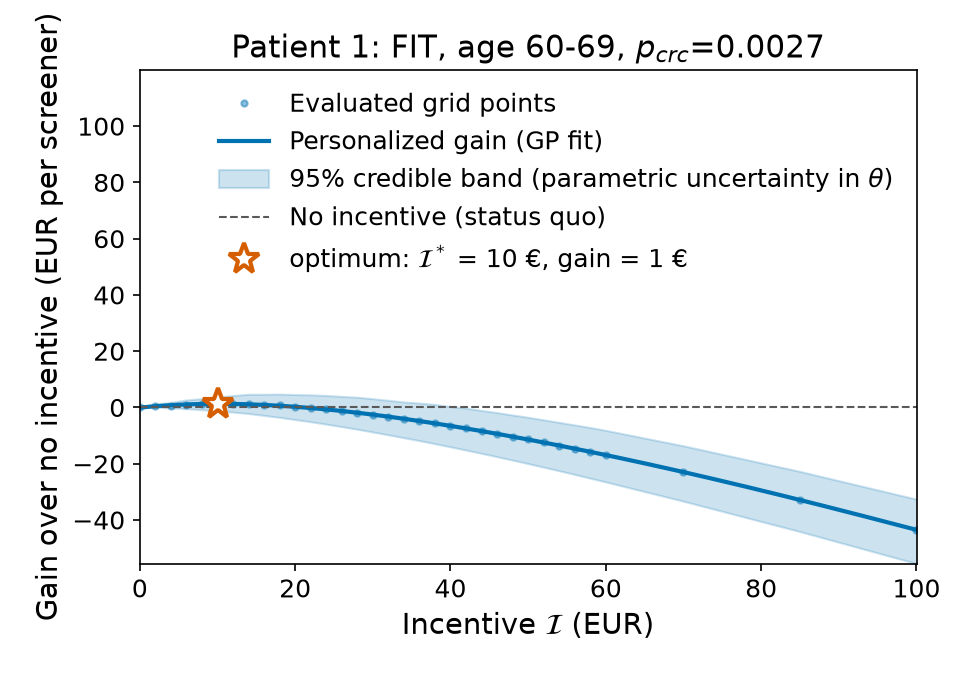
\includegraphics[width=\linewidth]{optimal_incentive_patient_1.png}
    \end{minipage}
    \begin{minipage}{0.325\textwidth}
        \centering
        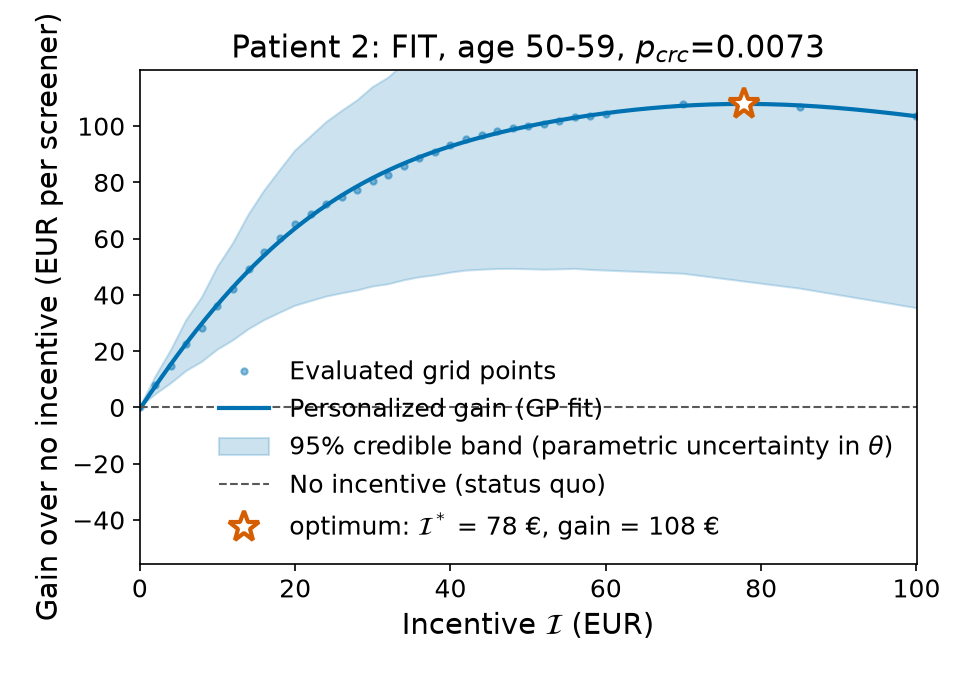
\includegraphics[width=\linewidth]{optimal_incentive_patient_2.png}
    \end{minipage}
    \begin{minipage}{0.325 \textwidth}
        \centering
        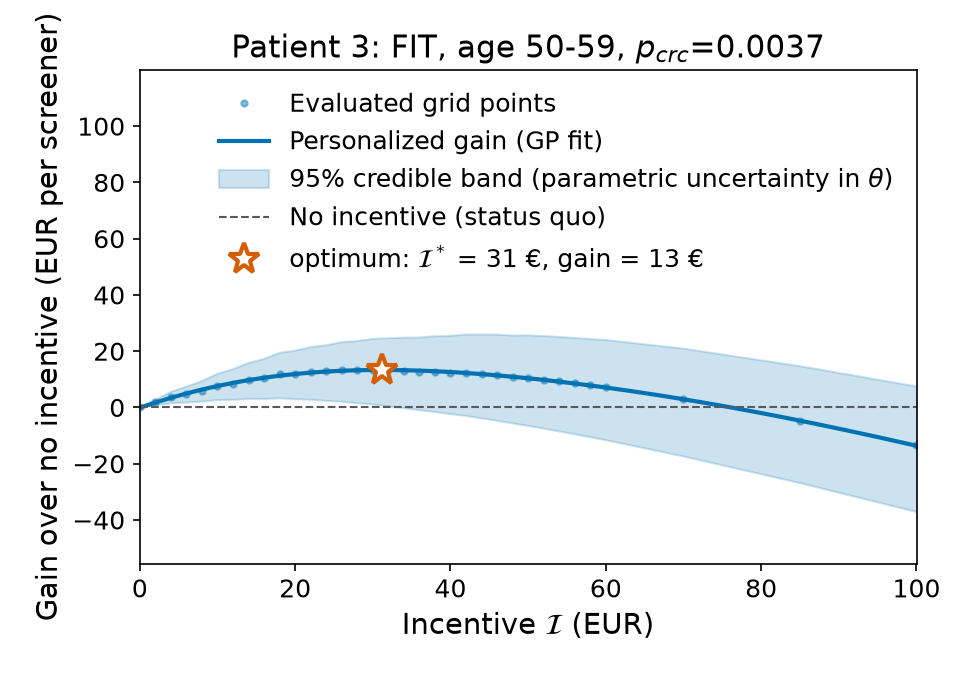
\includegraphics[width=\linewidth]{optimal_incentive_patient_3.png}
    \end{minipage}
    \caption{Optimal incentive for citizens 1, 2 and 3 of Table~\ref{tab:patients}. The dashed line at zero is the same citizen invited without incentive.}
    \label{fig:images_experiments}
\end{figure}

Table~\ref{tab:detection_gain} details the role of age in Section~\ref{sec:public_scheme_results}. The health value to the PM of detecting a cancer by screening rather than clinically, $(\bar\delta_{\text{cli}} - \bar\delta_{\text{scr}})\, \big[V^{PM}_{\text{future}}(0,x) - V^{PM}_{\text{future}}(1,x)\big] + \mathbb{E}[V^{PM}_{\text{treat}}(g,x) \mid \text{clinical}] - \mathbb{E}[V^{PM}_{\text{treat}}(g,x) \mid \text{screen}]$, doubles from ages 60--69 to 20--29, because younger citizens have more life-years to lose; the second term, the quality of life spared by treating an earlier stage, is worth 2{,}660€ at 60--69 and 2{,}910€ at 20--29, scaling with the age group's quality-of-life weight. Citizens perceive a smaller health value, discounted at $\lambda_C$ and weighted by present bias and risk perception, which also rises less steeply as age falls. Since the value of screening a citizen scales with their risk, however, and their risk falls faster with age than the value of a detection rises, younger citizens are both less valuable to screen and less willing to participate.
\begin{table}[h!]
\centering
\footnotesize
\caption{Health value of a screen-detected rather than clinically detected cancer, by age (€). Citizen: at $\lambda_C$, weighted by present bias and risk perception. Ratios relative to 60--69.}
\label{tab:detection_gain}
\begin{tabular}{c c r c r c}
\toprule
\textbf{Age} & $\bar Y$ & \textbf{PM} & \textbf{Ratio} & \textbf{Citizen, perceived} & \textbf{Ratio} \\
\midrule
20--29 & 59.5 & 108{,}076 & 1.99 & 32{,}587 & 1.64 \\
30--39 & 49.7 &  99{,}719 & 1.84 & 31{,}221 & 1.57 \\
40--49 & 40.0 &  86{,}908 & 1.60 & 28{,}480 & 1.43 \\
50--59 & 30.65 & 71{,}522 & 1.32 & 24{,}710 & 1.24 \\
60--69 & 21.9 &  54{,}227 & 1.00 & 19{,}858 & 1.00 \\
\bottomrule
\end{tabular}
\end{table}
\end{comment}


\bibliography{new_references}

\end{document}
